\documentclass[a4paper]{amsart}

\usepackage{a4wide} %A4 paper border

\usepackage{algorithm}
\usepackage[noend]{algpseudocode}

\usepackage{graphicx}
\usepackage{wrapfig}
\usepackage[usenames, dvipsnames, pdftex]{xcolor}
\usepackage[colorlinks=true,
        raiselinks=true,
        linkcolor=MidnightBlue,
        citecolor=ForestGreen,
        urlcolor=RoyalPurple,
        plainpages=false]{hyperref}

\usepackage{verbatim}
%% code snippets
\usepackage{listings}

\definecolor{classes}{HTML}{476A97}
\definecolor{methods}{HTML}{476A97}
\definecolor{comment}{HTML}{435138}
\definecolor{keywords}{HTML}{262C6A}
\definecolor{numbers}{HTML}{702C51}
\definecolor{strings}{HTML}{702C51}

\lstset{emph=[1]{%  
  clear,
  addByFunction,
  getInputs,
  getTransitionRelation,
  writeToFile,
  getSymbolicSet,
  setSymbolicSet,
  remPolytope,
  printInfo,
  mintermToElement,
  addPolytope,
  addEllipsoid,
  remEllipsoid,
  addGridPoints,
  complement,
  computeTransitionRelation,
  remGridPoints,
  addIndices,
  remIndices,
  fillAbstractSet,
  clearAbstractSet,
  xtoi,
  itox,
  minimalFixedPoint%
  },emphstyle=[1]{\color{methods}}%
}%

\lstset{emph=[3]{%
      size_t,input_t,state_t,%
    },emphstyle=[3]{\color{keywords}}%
}%

\lstset{emph=[2]{%
      INNER,
      OUTER,
      SymbolicSet, 
      SymbolicModel, 
      SymbolicModelGrowthBound,
      FixedPoint,
      UniformGrid,
      AbstractionGB,
      TransitionSystem%
    },emphstyle=[2]{\color{classes}}%
}%

% set the default code style
\lstset{
    columns=flexible,
    basicstyle=\ttfamily,
    frame=tb, % draw a frame at the top and bottom of the code block
    tabsize=2, % tab space width
    showstringspaces=false, % don't mark spaces in strings
    numbers=none, % display line numbers on the left
    commentstyle=\color{Gray}, % comment color
    keywordstyle=\color{keywords}, % keyword color
    stringstyle=\color{strings}, % string color
    language=C++,
}

\lstset{literate=%
    {scots::}{{{\color{classes}scots::}}}7
}


%\usepackage{parskip} % no paragraph indent

% math things
\usepackage{IEEEtrantools}
\usepackage[charter]{mathdesign}
\usepackage{amsmath} 
\usepackage{amsfonts}
\usepackage{amsthm}

% tikz
\usepackage{tikz}
\usetikzlibrary{arrows,automata}
\usetikzlibrary{shapes,snakes}
\usetikzlibrary{calc,positioning}


%% bibliography bibtex %.aux
\usepackage[
bibencoding=latin1,
sorting=none,
style=numeric-comp,
maxnames=3,
backend=biber
]{biblatex}
%\renewcommand*{\bibfont}{\raggedright}
\addbibresource{refs.bib}
%\renewcommand*{\bibfont}{\small}



%% custom commands 
%C plus plus
\newcommand\Cpp{C\texttt{++} }

\usepackage{stmaryrd}  % because of llbracket/rrbracket
\newcommand{\segcc}[1]{\ensuremath{{\left\llbracket#1\right\rrbracket}}}

%% begin: some math stuff
\newcommand{\intcc}[1]{\ensuremath{{\left[#1\right]}}}
\newcommand{\intoc}[1]{\ensuremath{{\left]#1\right]}}}
\newcommand{\intco}[1]{\ensuremath{{\left[#1\right[}}}
\newcommand{\intoo}[1]{\ensuremath{{\left]#1\right[}}}


\newcommand{\B}{\mathbb{B}}
\newcommand{\R}{\mathbb{R}}
\newcommand{\N}{\mathbb{N}}
\newcommand{\Z}{\mathbb{Z}}
\newcommand{\ul}{\underline}
\newcommand{\ol}{\overline}


\newcommand{\pre}{{\mathrm{pre}}}
\newcommand{\co}{{\mathrm{co}}}
\renewcommand{\emptyset}{{\varnothing}}
%% end: some math stuff





\title{SCOTS -- User Manual}

\author{Matthias Rungger}

\begin{document}
  \maketitle

	\tableofcontents
	\newpage
	

 

\part{INTRODUCTION}


\section{About {\tt SCOTS}}

{\tt SCOTS} is an open source software tool (available at
\mbox{\url{http://www.hcs.ei.tum.de}}) for the synthesis of 
symbolic controllers for possibly perturbed, nonlinear, control systems
according to~\cite{ReissigWeberRungger15}. It is mainly implemented
in \Cpp and it comes with a small MATLAB interface to access the synthesized controller
from within MATLAB. 

%Given a control problem
%$(S_1,\Sigma_1)$ consisting of a plant $S_1$ and a specification $\Sigma_1$, the
%synthesis scheme roughly proceeds as follows
%\begin{enumerate}
%  \item An auxiliary control problem $(S_2,\Sigma_2)$ is constructed.\\
%    Here $S_2$ is an \emph{symbolic model} (a.k.a.~\emph{abstraction}) and $\Sigma_2$
%    is an \emph{abstract specification}.
%  \item A controller $C$ for $S_2$, which solves the auxiliary controller problem
%    $(S_2,\Sigma_2)$ is computed.
%  \item The controller $C$ is \emph{refined} to a controller for $S_1$.
%\end{enumerate}

The tool is intended to be used and extended by researches in the area of formal methods for
cyber-physical systems. {\tt SCOTS} provides a baseline implementation of one of the most
basic approaches to symbolic synthesis. 

{\tt SCOTS} provides an implementation of the various algorithms using two
different data structures. One implementation is based on \emph{binary decision
diagrams} (BDD)~\cite{Bryant92} and one implementation is based on a sparse
matrix data structure {\color{red} (not yet included in the repository)}. 

%It can be used to compare the
%performance of more advanced algorithms with the basic implementation as well as  to rapidly 
%prototype extensions.

\section{Symbolic Controller Synthesis Basics}
\subsection{Control Problems} 
{\tt SCOTS} supports the computation of
controllers for  
nonlinear control systems of the form
\begin{IEEEeqnarray}{c}\label{e:System:c-time}
\dot \xi(t) \in f(\xi(t),u) + \segcc{-w,w}
\end{IEEEeqnarray}
where $f$ is given by \mbox{$f:\mathbb{R}^n\times U\to \mathbb{R}^n$} and
$U\subseteq \R^m$. The vector $w=\intcc{w_1,\ldots,w_n}\in \mathbb{R}_+^n$ is a perturbation
bound and $\segcc{-w,w}$ denotes the hyper-interval
$\intcc{-w_1,w_1}\times\ldots\times \intcc{-w_n,w_n}$. Given a  time horizon $\tau>0$, we define a \emph{solution
of~\eqref{e:System:c-time} on $\intcc{0,\tau}$ under (constant) input
\mbox{$u\in U$}} 
as an absolutely continuous function \mbox{$\xi \colon \intcc{0,\tau}
\to \mathbb{R}^n$} that satisfies
\eqref{e:System:c-time} for almost every (a.e.) \mbox{$t \in
\intcc{0,\tau}$}.


The desired behavior of the closed loop is defined with respect to the
$\tau$-sampled behavior of the continuous-time systems~\eqref{e:System:c-time}.
To this end, the sampled behavior of~\eqref{e:System:c-time} is casted as
\emph{simple system}~\cite{ReissigWeberRungger15} 
\begin{IEEEeqnarray}{c}
  S_1:=(X_1,U_1,F_1)
\end{IEEEeqnarray}
with the \emph{state alphabet} $X_1:=\R^n$, \emph{input alphabet} $U_1:=U$ and
the \emph{transition function} $F_1:X_1 \times U_1\rightrightarrows X_1$ defined
by 
\begin{IEEEeqnarray*}{c}
  F_1(x,u):=\{x'\mid \exists_{ \text{$\xi$ is a solution of~\eqref{e:System:c-time} on
  $\intcc{0,\tau}$ under $u$}}: \xi(0)=x \land \xi(\tau)=x'\}.
\end{IEEEeqnarray*}
A \emph{specification} $\Sigma_1$ for a simple system $S_1=(X_1,U_1,F_1)$ is
simply a set 
\begin{IEEEeqnarray}{c}
  \Sigma_1\subseteq \bigcup_{T\in \Z_{\ge0}\cup \{\infty\}}(U_1\times
  X_1)^{\intco{0;T}} =: (U_1\times X_1)^\infty
\end{IEEEeqnarray}
of possibly finite and infinite input-state sequences.
A simple system $S_1$ together with a specification $\Sigma_1$ constitute an
\emph{control problem} $(S_1,\Sigma_1)$.

{\tt SCOTS} natively supports invariance (often referred to as safety)  and
reachability specifications. Consider two sets $I_1\subseteq X_1$ and
$Z_1\subseteq X_1\times U_1 $.
A \emph{reachability} specification associated
with $I_1,Z_1$ is defined by
\begin{IEEEeqnarray*}{c}
  \Sigma_1:=\{(u,x)\in (U_1\times X_1)^\infty
  \mid  x(0)\in I_1\implies \exists_{t\in\intco{0;T}}: (x(t),u(t))\in Z_1\}.
\end{IEEEeqnarray*}
An
\emph{invariance} specification associated with $I_1,Z_1$ follows by 
\begin{IEEEeqnarray*}{c}
\Sigma_1:=\{(u,x)\in (U_1\times X_1)^{\intco{0;\infty}} \mid x(0)\in I_1\implies
\forall_{t\in\intco{0;\infty}}: (x(t),u(t))\in Z_1\}.
\end{IEEEeqnarray*}
In this context, the sets $I_1$ and $Z_1$ are referred to as \emph{atomic
propositions}.
\texttt{SCOTS} allows to define arbitrary sets as atomic propositions. In the BDD implementation, it provides
customized commands to define 
\begin{itemize}
\item polytopes $\{x\in \R^n\mid Hx \le h\}$ parameterized by $H\in\R^{q\times n}$,
$h\in\R^q$, and 
\item ellipsoids $\{x\in\R^n\mid |L(x-y)|_2\le 1\}$ parameterized by
$L\in\R^{n\times n}$ and $y\in\R^n$.
\end{itemize}
It is also possible to synthesize
controllers with respect more general specifications such as 
\begin{itemize}
  \item \emph{reach-and-stay}, see the example in {\tt\small
    ./examples/bdd/dcdc2/} and Sec.~\ref{ss:controllersynthesis}.
  \item \emph{reactivity} {\color{red} (not yet included)}.
\end{itemize}



\subsection{Auxiliary Control Problems}
\label{ss:symbolicmodel}

Given a simple system $S_1=(X_1,U_1,F_1)$ representing the $\tau$-sampled
behavior of~\eqref{e:System:c-time} and a specification $\Sigma_1$ for $S_1$,
the control problem $(S_1,\Sigma_1)$ is not solved directly, but an auxiliary,
finite control problem $(S_2,\Sigma_2)$ is used in the synthesis process. Here, 
$S_2=(X_2,U_2,F_2)$ is a  \emph{symbolic model} or (discrete)
\emph{abstraction} of $S_1$ and $\Sigma_2$ is an abstract specification.

The state alphabet of $X_2$ is a cover of $X_1$ and the input alphabet $U_2$ is
a subset of $U_1$. The set $X_2$ contains a subset $\bar X_2$, representing the ``real'' quantizer symbols,
while the remaining symbols $X_2\smallsetminus \bar X_2$ are interpreted as
``overflow'' symbols. The set of real quantizer symbols $\bar X_2$ are given by
congruent hyper-rectangles aligned on a uniform grid 
\begin{IEEEeqnarray}{c}
\label{e:grid}
  \eta\Z^n=\{c\in \R^n\mid \exists_{k\in\Z^n}\forall_{i\in\intcc{1;n}}\; c_i=k_i\eta_i\}
\end{IEEEeqnarray}
with \emph{grid parameter} $\eta\in(\R_+\smallsetminus\{0\})^n$, i.e., 
\begin{IEEEeqnarray}{c}\label{e:abs:ss}
  x_2\in \bar X_2\implies \exists_{c\in \eta\Z^n}\;x_2=c+\segcc{-\eta/2,\eta/2}.
\end{IEEEeqnarray}
{\tt SCOTS} computes symbolic models that are related via feedback
refinement relations with the plant. A \emph{feedback refinement relation} from
$S_1$ to $S_2$ is a strict relation $Q\subseteq X_1\times X_2$ that satisfies
for all $(x_1,x_2)\in Q$ and for all $u\in U_2$ with $F_2(x_2,u)\neq\emptyset$
the conditions
\begin{enumerate}
  \item $F_1(x_1,u)\neq \emptyset$ and
  \item $Q(F_1(x_1,u))\subseteq F_2(x_2,u)$.
\end{enumerate}
In {\tt SCOTS}, the feedback refinement relation $Q$ is given by the set-membership
relation
\begin{IEEEeqnarray}{c}
  Q:=\{ (x_1,x_2) \mid x_1 \in x_2\}.
\end{IEEEeqnarray}
Given an invariance (reachability) specification $\Sigma_1$ for $S_1$ associated with
$(I_1,Z_1)$ an \emph{abstract specification} is given by the invariance
(reachability) specification for $S_2$ associated with 
\begin{IEEEeqnarray}{c't'c}
  I_2=\{ x_2 \in X_2\mid x_2\cap I_1\neq\emptyset\} & and & Z_2=\{ x_2 \in
X_2\mid x_2\subseteq  Z_1\neq\emptyset\}.
\end{IEEEeqnarray}
For the solution of the auxiliary control problems $(S_2,\Sigma_2)$ {\tt SCOTS}
provides minimal and maximal fixed point algorithms~\cite{RunggerZamani16}.


\subsection{Growth Bound}
\label{ss:GB} 

The construction of a symbolic model $S_2$ of $S_1$
is based on the over-approximation of
attainable sets. To this end, we use the notion of a growth bound
introduced in~\cite{ReissigWeberRungger15}.
A \emph{growth bound} of~\eqref{e:System:c-time} is a function $\beta \colon
\mathbb{R}_{+}^n \times U' \to \mathbb{R}_{+}^n$, which is defined with respect to a sampling time
$\tau>0$, a set $K\subseteq \mathbb{R}^n$ and a set $U'\subseteq U$.
Basically, it provides an upper bound on the deviation of solutions $\xi$
of~\eqref{e:System:c-time} from \emph{nominal
solutions}\footnote{A nominal solution $\varphi(\cdot,p,u)$ of
\eqref{e:System:c-time} is defined as solution of the initial value problem $\dot x=f(x,u)$,
$x(0)=p$.} $\varphi$ of~\eqref{e:System:c-time}, i.e., for every solution $\xi$ of \eqref{e:System:c-time} on $\intcc{0,\tau}$ with input $u \in U'$ and $\xi(0),p \in K$,
we have
\begin{IEEEeqnarray}{c}
\label{e:growthbound}
| \xi(\tau) - \varphi(\tau,p,u) | \leq \beta( | \xi(0) - p |, u).
\end{IEEEeqnarray}
Here, $|x|$ for $x\in\R^n$, denotes the component-wise absolute value.
A growth bound can be obtained essentially by bounding
the Jacobian of $f$. Let
$L \colon U' \to \mathbb{R}^{n \times n}$ satisfy
\begin{IEEEeqnarray}{c}\label{e:lipschitz}
L_{i,j}(u)
\geq
\begin{cases}
D_j f_i(x,u)& \text{if $i=j$,}\\
| D_j f_i(x,u) |& \text{otherwise}
\end{cases}
\end{IEEEeqnarray}
for all $x\in K'\subseteq \R^n$ and $u\in U'\subseteq U$. Then 
\begin{IEEEeqnarray}{c}
\label{e:GrowthBoundComputation}
\beta(r,u)
=
e^{L(u)\tau}
r
+
\int_0^\tau
e^{L(u)s}
w
\;\mathrm{d}s,
\end{IEEEeqnarray}
is a growth bound on $\intcc{0,\tau}$, $K$, $U'$
associated with \eqref{e:System:c-time}. The domain $K'$ on
which~\eqref{e:lipschitz} needs to hold, is assumed to be convex and contain any
solution $\xi$ on $\intcc{0,\tau}$ of~\eqref{e:System:c-time} with $u\in U'$ and
$\xi(0)\in K$,
see~\cite[Thm.~VIII.5]{ReissigWeberRungger15}. 

In order to use {\tt SCOTS}, the user needs to provide a growth bound, which for
nonlinear control systems can be provided in terms of the parameterized matrix
$L(u)$ whose entries satisfy~\eqref{e:lipschitz}.

%of $S_1$, i.e., a simple system which is related via \emph{feedback refinement
%relation} $Q\subseteq X_1\times X_2$. 
%
%The controller synthesis algorithms implemented in {\tt SCOTS} are based on
%certain finite representations, often termed 
%\cite{MoorRaisch99}, of
% continuous control systems. {\tt SCOTS} supports the computation of symbolic
%models of the $\tau$-sampled behavior of perturbed, 

\subsection{Closed Loop} 

The \emph{solution} of a control problem $(S,\Sigma)$ is a \emph{system}  $C=(X_c,X_{c,0},U_c,V_c,Y_c,F_c,H_c)$ which is \emph{feedback composable} with
$S_1$, see~\cite[Def.~III.3]{ReissigWeberRungger15}, so that 
\begin{IEEEeqnarray*}{c}
  \mathcal{B}(C\times S)\subseteq \Sigma.
\end{IEEEeqnarray*}
Here $\mathcal{B}(C\times S)$ denotes the \emph{behavior} of the closed
loop $C\times S_1$, see~\cite[Def.~V.1]{ReissigWeberRungger15}. 
The main statement enabling the symbolic synthesis approach reads as
follows~\cite[Thm.~VI.3]{ReissigWeberRungger15}.

\emph{Consider two control problems $(S_i,\Sigma_i)$, $i\in\{1,2\}$. Suppose that $Q$
is a feedback refinement relation from $S_1$ to $S_2$ and $\Sigma_2$ is an
abstract specification of $\Sigma_1$. If $C$ solves the control problem $(S_2,\Sigma_2)$, then $C\circ
Q$ solves the control problem $(S_1,\Sigma_1)$.}

The controller $C\circ Q$ for $S_1$ is given by the serial composition of the quantizer
$Q:X_1\rightrightarrows X_2$ with the controller $C$. 
The closed loop resulting from a simple system $\Sigma_1$ which represents the $\tau$-sampled
behavior of~\eqref{e:System:c-time} and a controller $C\circ Q$ is illustrated
in Fig.~\ref{f:closedloop}. At each $k\in\Z_{\ge0}$ sampling
time $\tau>0$, the plant state $x_1=\xi(k\tau)$ is measured and fed to the
quantizer $Q$, which is used to determine a cell $x_2\in X_2$ that contains
$x_1\in x_2$. Then $x_2$ is feed to the controller $C$ to pick the input $u\in
U_2\subseteq U_1$ which is applied to~\eqref{e:System:c-time}.
\begin{figure}[h]
  \centering
  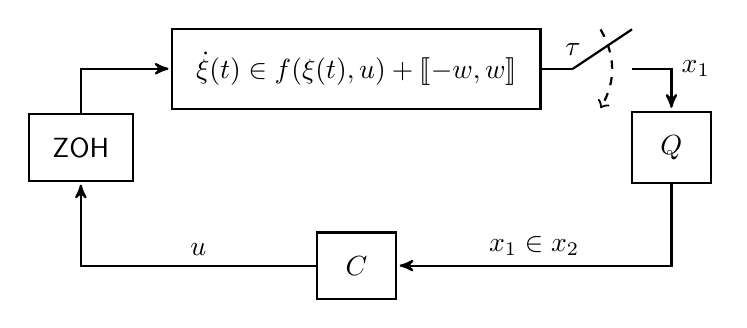
\begin{tikzpicture}
    [
    mynode/.style={draw,
                   thick,
                   inner sep=.3cm,
                   minimum width=1cm},
    %
    to/.style={->,
               >=stealth',
               shorten >=1pt,
               thick},
    ]

    \node [mynode] (sys) at (0,0) {$\dot \xi(t)\in f(\xi(t),u)+\segcc{-w,w}$};
    \node [mynode] (con) at (0,-2.5) {$C$};
    \node [mynode] (zoh) at (-3.5,-1) {$\mathsf{ZOH}$};

    %\node [mynode] (dist) at (4,0) {$P$};
    \node [mynode] (quant) at (4,-1) {$Q$};

    \node at (2.75,0.25) {$\tau$};


    \draw [to]  (zoh.north) |-  (sys.west);
    \draw [to]  (con.west)  -| node[above, near start] {$u$} (zoh.south);

    \draw[to] (3.5,0) -| node[right] {$x_1$} (quant.north);
    \draw[to] (quant.south) |- node[above, near end] {$x_1\in x_2$} (con.east);

    \draw[thick] (sys.east) -- (2.75,0);
    \draw[thick] (2.75,0) -- (3.5,.5);
    \draw[dashed,thick,bend left,->] (3.1,.5) to (3.1,-.5);

  \end{tikzpicture}
\caption{Sample-and-hold implementation of a controller synthesized with {\tt SCOTS}.}\label{f:closedloop}
\end{figure}

%In case that
%$\Sigma_1$ is an invariance or a reachability specification, the solution $C$ is
%a \emph{static} system, which means that the state alphabet is a singleton, i.e.,
%$X_c=\{x_c\}$. The output function 
%
%In the simplest
%case, $C$ is a \emph{static} system, which means $X_c$

Additionally to the perturbations on the right-hand-side
of~\eqref{e:System:c-time}, it is possible to account for measurement errors
modeled by a set-valued map $P \colon \mathbb{R}^n \rightrightarrows
\mathbb{R}^n$ given by
\begin{IEEEeqnarray}{c't'c}\label{e:perturbation}
  P(x):=x+\segcc{-z,z} & with & z\in\R_+^n.
\end{IEEEeqnarray}
Please see~\cite[Sec.~VI.B]{ReissigWeberRungger15} and~\cite{RunggerZamani16}
for some background theory.
The closed loop with measurement errors is illustrated
in~Fig.~\ref{f:closedloop:pert}.
\begin{figure}[h]
\centering
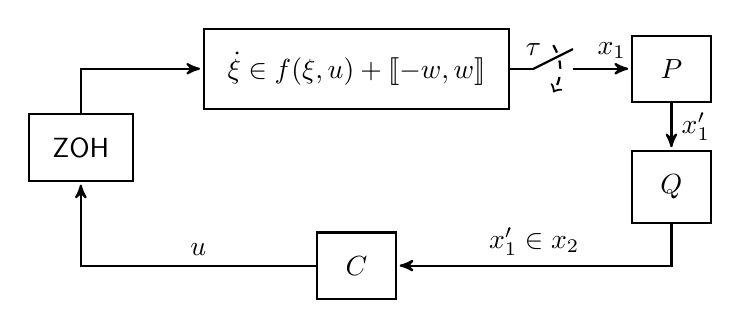
\begin{tikzpicture}
  [
  mynode/.style={draw,
                 thick,
                 inner sep=.3cm,
                 minimum width=1cm},
  %
  to/.style={->,
             >=stealth',
             shorten >=1pt,
             thick},
  ]

  \node [mynode] (sys) at (0,0) {$\dot \xi\in f(\xi,u)+\segcc{-w,w}$};
  \node [mynode] (con) at (0,-2.5) {$C$};

  \node [mynode] (zoh) at (-3.5,-1) {$\mathsf{ZOH}$};

  \node [mynode] (dist) at (4,0) {$P$};
  \node [mynode] (quant) at (4,-1.5) {$Q$};

  \node at (2.25,0.25) {$\tau$};


  \draw[thick] (sys.east) -- (2.25,0);
  \draw[thick] (2.25,0) -- (2.75,.25);
  \draw[dashed,thick,bend left,->] (2.5,.3) to (2.5,-.3);
  \draw[thick] (2.75,0) -- (3,0);

  \draw[to] (3,0) -- node[above] {$x_1$} (dist.west);
  \draw[to] (dist.south) -- node[right] {$x_1'$} (quant.north);


  \draw [to]  (zoh.north) |-  (sys.west);
  \draw [to]  (con.west)  -| node[above, near start] {$u$} (zoh.south);

  \draw[to] (quant.south) |- node[above, near end] {$x'_1\in x_2$} (con.east);

\end{tikzpicture}
\caption{Closed loop with measurement errors modeled by the set-valued map $x'_1 \in P(x_1)$.}\label{f:closedloop:pert}
\end{figure}


\subsection{Synthesis via Fixed Point Computations}
\label{ss:fixedpoint}
For the synthesis of controllers $C$ to enforce reachability, respectively,
invariance specifications,
\texttt{SCOTS} provides two fixed point algorithms.


Consider $S_2=(X_2,U_2,F_2)$ with $X_2$ finite and $I_2\in X_2$, $Z_2\subseteq
X_2\times U_2$. For $Y\subseteq X_2\times U_2$, we 
define the map 
\begin{IEEEeqnarray}{c}\label{e:pre}
  \pre(Y):=\{(x_2,u)\in X_2\times U_2\mid  F_2(x_2,u)\neq \emptyset \land
  F_2(x_2,u)\subseteq\pi_{X_2}(Y)\}.
\end{IEEEeqnarray}
where $\pi_{X_2}(Y)$ denotes the projection of $Y$ onto $X_2$.

We compute a controller to enforce a reachability specification $\Sigma_2$
associated with $I_2,Z_2$, by computing the minimal fixed point of the map
$Y\mapsto \pre(Y)\cup Z_2$, which we denote by using the usual $\mu$ calculus
notation~\cite{ArnoldNiwinski01} as
\begin{IEEEeqnarray*}{c}
  \mu Y. \pre(Y)\cup Z_2.
\end{IEEEeqnarray*}
In order to extract a controller, we introduce the function $j:X_2\to\N\cup\{\infty\}$ by
\begin{IEEEeqnarray*}{c}
j(x)=\inf\{i\in \N\mid x\in \pi_{X_2}(Y_i)\}
\end{IEEEeqnarray*}
where the sets $Y_i$ are recursively given by
\begin{IEEEeqnarray*}{rCl}
	Y_0&=&\emptyset\\
	Y_{i+1}&=&\pre(Y_i)\cup Z_2.
\end{IEEEeqnarray*}
Of course we have $Y_i=Y_{i+1}$ implies $Y_i=\mu Y. \pre(Y)\cup Z_2$. Let use define the map
\begin{IEEEeqnarray}{rCl}\label{e:con:reach}
	H'_c(x_2)=\big\{u\in U\mid (x_2,u)\in Z_2 \vee ( F_2(x_2,u)\neq \emptyset \land F_2(x_2,u)\subseteq \pi_{X_2}(Y_{j(x_2)-1}))\big\}
\end{IEEEeqnarray}
which is non-empty for all $x_2\in \mu Y.\pre(Y)\cup Z_2$.
We derive a controller as a system
according to~\cite[Def.~III.1]{ReissigWeberRungger15} (ver.~2) by $C=(\{q\},\{q\},X_2,X_2,U_2,F_c,H_c)$ with 
\begin{IEEEeqnarray*}{rCl}
H_c(q,x_2)&=&
\begin{cases}
H'_c(x_2)\times \{x_2\} & \text{if } x_2\in \mu Y. \pre(Y)\cup Z_2\\
U_2\times\{x_2\} & \text{otherwise}
\end{cases}\\
F_c(q,x_2)&=&
\begin{cases}
\{q\} & \text{if } x_2\in \mu Y. \pre(Y)\cup Z_2\\
\emptyset &  \text{otherwise}
\end{cases}
\end{IEEEeqnarray*}


Similarly, if
$\Sigma_2$ is an invariance specification associated with $I_2,Z_2$, we compute the maximal fixed point of $Y\mapsto \pre(Y)\cap Z_2$, which is denoted by
\begin{IEEEeqnarray*}{c}
  \nu Y. \pre(Y)\cap Z_2.
\end{IEEEeqnarray*}
Given $\nu Y. \pre(Y)\cap Z_2$ we define the map
\begin{IEEEeqnarray}{rCl}\label{e:con:inv}
	H'_c(x_2)=\big\{u\in U\mid F_2(x_2,u)\neq \emptyset \land F_2(x_2,u)\subseteq \pi_{X_2}(\nu Y. \pre(Y)\cap Z_2)\big\}.
\end{IEEEeqnarray}
and the controller 
according to~\cite[Def.~III.1]{ReissigWeberRungger15} (ver.~2) follows again by
\begin{IEEEeqnarray*}{rCl}
H_c(q,x_2)&=&
\begin{cases}
H'_c(x_2)\times \{x_2\} & \text{if } x_2\in \nu Y. \pre(Y)\cap Z_2\\
U_2\times\{x_2\} & \text{otherwise}
\end{cases}\\
F_c(q,x_2)&=&
\begin{cases}
\{q\} & \text{if } x_2\in \nu Y. \pre(Y)\cap Z_2\\
\emptyset &  \text{otherwise}
\end{cases}
\end{IEEEeqnarray*}
In either case, it is well known~\cite{Tabuada09} that $C$ solves the control problem
$(S_2,\Sigma_2)$ with $\Sigma_2$ being a reachability (invariance)
specification iff $I_2\subseteq \pi_{X_2}(\mu Y.\pre(Y)\cup Z_2)$  ($I_2\subseteq \pi_{X_2}(\nu Y.\pre(Y)\cap Z_2)$).
Also for both types of specifications the controller is \emph{memoryless} or
\emph{static}, i.e., the output is independent of the state.





\newpage
\section{Source Code Organization}


\begin{lstlisting}[basicstyle=\small\ttfamily]

./bdd  									/* the source code of the BDD based implementation */ 
./doc                   /* the C++ class documentation created with NaturalDocs */
./examples             	/* directory containing various examples */ 
./examples/hscc16      	/* examples presented at HSCC16 using the BDD impl. */ 
./license.txt						/* the license file */
./manual 								/* directory containing this manual */
./mfiles 								/* the MATLAB files */
./mfiles/mexfiles 			/* mex files to access the controller from MATLAB */
./readme.txt           	/* a quick description pointing to this manual */
./sparse								/* the source code of the sparse matrix implementation */
./utils 								/* some helper code */

\end{lstlisting}

\section{Installation}
\label{s:req}

In general, {\tt SCOTS} is implemented in ``header-only'' style and you only
need a working \Cpp developer environment. However, the BDD based
implementation uses the {\tt CUDD} library by Fabio Somenzi, which can be downloaded at
  \url{http://vlsi.colorado.edu/~fabio/}. 
Moreover, for the illustration of atomic propositions as well as for the closed
loop simulation a MATLAB interface and, hence, a working installation of MATLAB is needed.  

The requirements are summarized as follows:

\begin{enumerate}
  \item A working C/\Cpp{} development environment
    \begin{itemize}
      \item Mac OS X: You should install Xcode.app including the command line tools
      \item Linux: Most linux OS include the necessary tools already
      \item Windows: We haven't tested the code with Windows
    \end{itemize}

  \item A working installation of the {\tt CUDD} library with 
     \begin{itemize}
      \item the \Cpp{} object-oriented wrapper
      \item the dddmp library and
      \item the shared library 
    \end{itemize}
   option enabled. The package follows the usual {\tt \small configure}, {\tt
   \small make} and
   {\tt \small make install} installation routine. We use {\tt \small cudd-3.0.0}, with the
   configuration
\begin{lstlisting}[basicstyle=\small\ttfamily,frame=none]
  $ ./configure --enable-shared --enable-obj --enable-dddmp --prefix=/opt/local/
\end{lstlisting}
You should test the BDD installation by compiling a dummy
programm, e.g. {\tt \small test.cc} 
\begin{lstlisting}[basicstyle=\footnotesize\ttfamily]
#include<iostream>
#include "cuddObj.hh"
#include "dddmp.h"
int main () {
  Cudd mgr(0,0);
  BDD x = mgr.bddVar();
}
\end{lstlisting}
should be compiled by
\begin{lstlisting}[basicstyle=\small\ttfamily,frame=none]
  $ g++ test.cc -I/opt/local/include -L/opt/local/lib -lcudd
\end{lstlisting}
On some linux machines we experienced that the header files {\tt \small util.h} and
{\tt \small config.h} were missing in {\tt \small /opt/local} and we manually
copied them to {\tt \small /opt/local/include}.

  \item A recent version of MATLAB. We conducted
  the experiments with version {\tt \small R2015b (8.6.0.232648) 64-bit (maci64)}.
  To compile the mex files:
  \begin{enumerate}
    \item open MATLAB and setup the mex compiler by
  \begin{lstlisting}[basicstyle=\small\ttfamily,frame=none]
     >> mex -setup C++
  \end{lstlisting}
      \item edit the {\tt \small Makefile}  and adjust the variables
      \begin{itemize}
        \item {\tt \small MATLABROOT} and {\tt \small CUDDPATH}
      \end{itemize}
    \item in a terminal run
      {\tt \small \$ make}
  \end{enumerate}
\end{enumerate}
	

\part{BDD BASED IMPLEMENTATION}
  


\section{Quickstart}

For a quickstart 
\begin{enumerate}
	\item go to one of the examples in
	\begin{lstlisting}[basicstyle=\footnotesize\ttfamily]
	./examples/hscc16/dcdc      			/* invariance specification */ 
	./examples/hscc16/vehicle2      	/* reachability specification */ 
  ./examples/bdd/dcdc2      				/* reach-and-stay specification */ 
  ./examples/bdd/boostsolver 		   	/* using an ODE solver form the BOOST lib */ 
	\end{lstlisting}
	\item read the readme file (if the directory contains one)
	\item edit the {\tt \small Makefile} 
	\begin{enumerate}
		\item adjust the compiler
		\item adjust the directories of the CUDD library 
 \end{enumerate}
	\item compile and run the executable, for example in  {\tt \small ./examples/hscc16/dcdc} run
\begin{lstlisting}[basicstyle=\small\ttfamily,frame=none]
	$ make
	$ ./dcdc 
\end{lstlisting}
  \item open MATLAB (here we assume that you have already compiled the mex files)
    and add {\tt \small ./mfiles} to the MATLAB path 
\begin{lstlisting}[basicstyle=\small\ttfamily,frame=none]
  >> addpath(genpath('../../../mfiles')) 
\end{lstlisting}
  \item run the m file, for example in  {\tt \small ./examples/hscc16/dcdc} run
\begin{lstlisting}[basicstyle=\small\ttfamily,frame=none]
	>> dcdc
\end{lstlisting}
\item modify the example to your needs
\end{enumerate}




\section{Work Flow Overview}

A short description of the general work flow is given by
\begin{enumerate}
  \item Use the class {\tt\small SymbolicSet} to specify 
    \begin{itemize}
      \item the real quantizer symbols $\bar X_2$ 
      \item the input alphabet $U_2$ 
    \end{itemize}
  \item Use the class {\tt\small SymbolicModelGrowthBound} to compute 
the transition function $F_2$. You
need to provide 
    \begin{itemize}
      \item the solution of the right-hand-side~\eqref{e:System:c-time} at time $\tau$
      \item and the growth bound~\eqref{e:growthbound} (directly or in terms of $L(u)$
    see~\eqref{e:lipschitz})
    \end{itemize}
  \item Use { \tt\small SymbolicSet} to specify the atomic propositions
    in the specification
  \item Use { \tt \small FixedPoint} to solve the auxiliary control problem $(S_2,\Sigma_2)$ 
  \item Use { \tt\small SymbolicSet}  to write the result to a file
  \item Optional: Simulate the closed loop in MATLAB by accessing the
    controller saved in the file
\end{enumerate}

An overview of the usage is illustrated in Fig.~\ref{f:usage}. 

\begin{figure}[th]
\centering
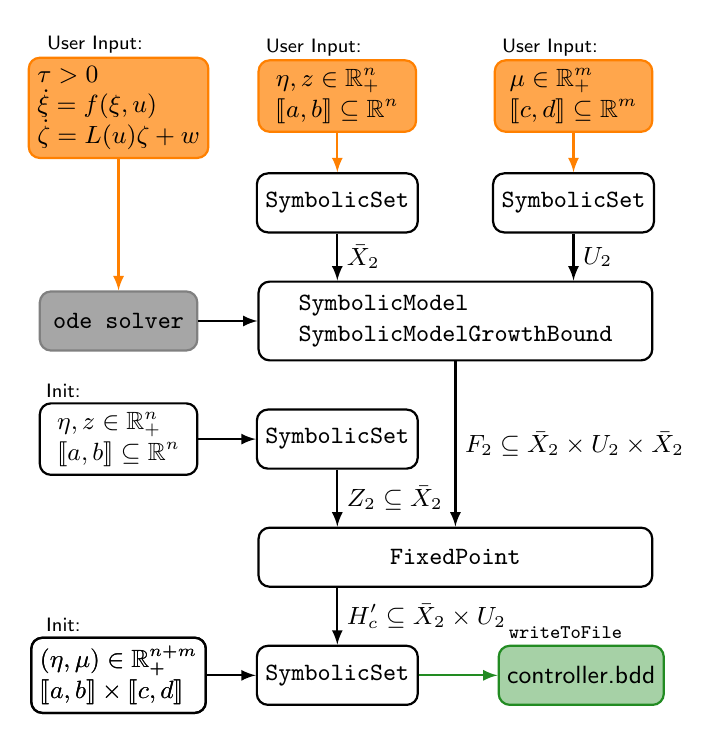
\begin{tikzpicture}
[>=latex,
ui/.style={draw=orange, thick, fill = orange!70!white, align=left, rounded corners, minimum height=.75cm, minimum width=2cm},
thirdparty/.style={draw=gray, thick, fill = gray!70!white, align=left, rounded corners, minimum height=.75cm, minimum width=2cm},
uic/.style={draw=orange}
]
\small
%% state space start
\node[draw,
      thick,
      rounded corners,
      minimum height=.75cm,
      minimum width=2cm] (ss) at (0,0) {\texttt{SymbolicSet}};

\node[ui, above = .5cm of ss] (uiss)  {$\eta,z\in \R_{+}^n$\\$\segcc{a,b}\subseteq \R^n$};

\draw[uic,thick,->] (uiss.south) -- (ss.north);
\node at ($(uiss.north)+(-0.3,.15)$) {{\scriptsize{\sf User Input:}}};
%% state space ned

%% input space start
\node[draw,
      thick,
      rounded corners,
      minimum height=.75cm,
      minimum width=2cm] (is) at (3,0) {\texttt{SymbolicSet}};

\node[ui, above = .5cm of is] (uiis)  {$\mu\in \R_{+}^m$\\$\segcc{c,d}\subseteq \R^m$};

\draw[uic,thick,->] (uiis.south) -- (is.north);
\node at ($(uiis.north)+(-0.3,.15)$) {{\scriptsize{\sf User Input:}}};
%% input space end

%% symbolic model start
\node[draw,
      thick,
      rounded corners,
      align=left,
      minimum height=1cm,
      minimum width=5cm] (sm) at (1.5,-1.5) {\texttt{SymbolicModel}\\\texttt{SymbolicModelGrowthBound}};

\node[thirdparty, left = .75cm of sm] (ode)  {\texttt{ode solver}};

\draw[thick,->] (ode.east) -- (sm.west);

\node[ui] at ($(uiss -| ode)+(0,-.15)$) (uism)  {$\tau>0$\\$\dot \xi=f(\xi,u)$\\$\dot \zeta=L(u)\zeta+w$};
\node at ($(uism.north)+(-0.3,.15)$) {{\scriptsize{\sf User Input:}}};

\draw[uic,thick,->] (uism.south) -- (ode.north);


\draw[thick,->] (is.south) -- node[right] {$U_2$} (is |- sm.north);
\draw[thick,->] (ss.south) -- node[right] {$\bar X_2$} (ss |- sm.north);
%% symbolic model end

%% fixed point start
\node[draw,
      thick,
      rounded corners,
      minimum height=.75cm,
      minimum width=2cm] (fpss) at (0,-3) {\texttt{SymbolicSet}};

\node[draw,
      thick,
      align=left,
      rounded corners,
      minimum height=.75cm,
      minimum width=2cm] (uifp) at (fpss -| ode)  {$\eta,z\in \R_{+}^n$\\$\segcc{a,b}\subseteq \R^n$};
\node at ($(uifp.north)+(-0.7,.15)$) {{\scriptsize{\sf Init:}}};


\draw[thick,->] (uifp.east) -- (fpss.west);

\node[draw,
      thick,
      rounded corners,
      align=left,
      minimum height=.75cm,
      minimum width=5cm] (fp) at (1.5,-4.5) {\texttt{FixedPoint}};

\draw[thick,<-] (fp.north) -- node[right] {$F_2\subseteq \bar X_2\times U_2\times \bar X_2$} (fp |- sm.south);
\draw[thick,->] (fpss.south) -- node[right] {$Z_2\subseteq \bar X_2$} (fpss |- fp.north);
%% fixed point end

%% fixed point output start
\node[draw,
      thick,
      rounded corners,
      minimum height=.75cm,
      minimum width=2cm] (con) at (0,-6) {\texttt{SymbolicSet}};

\draw[thick,<-] (con.north) -- node[right] {$H_c'\subseteq \bar X_2\times U_2$} (con |- fp.south);

\node[draw=ForestGreen,
      thick,
      right = of con,
      fill=ForestGreen!40,
      rounded corners,
      minimum height=.75cm,
      minimum width=2cm] (out) {\textsf{controller.bdd}};
\node at ($(out.north)+(-0.2,.15)$) {{\scriptsize{\tt writeToFile}}};

\draw[thick,draw=ForestGreen,->] (con) -- (out) ;


\node[draw,
      thick,
      align=left,
      rounded corners,
      minimum height=.75cm,
      minimum width=2cm] (ic) at (uifp |- con)  {$(\eta,\mu)\in \R_{+}^{n+m}$\\$\segcc{a,b}\times \segcc{c,d}$};
\node at ($(ic.north)+(-0.7,.15)$) {{\scriptsize{\sf Init:}}};
\draw[thick,->] (ic) --  (con);

\node[draw=,
      thick,
      align=left,
      rounded corners,
      minimum height=.75cm,
      minimum width=2cm] (ic) at (uifp |- con)  {$(\eta,\mu)\in \R_{+}^{n+m}$\\$\segcc{a,b}\times \segcc{c,d}$};

%% fixed point output end


%%%% cudd box start
%%\node[draw=green!20!black,
%%      thick,
%%      fill=green!20!white,
%%      rounded corners,
%%      minimum height=.75cm,
%%      minimum width=1cm] (cudd) at (uism |- uiss)  {\texttt{Cudd}};
%%%% cudd box 
\end{tikzpicture}%
\caption{The work flow in \texttt{SCOTS}.}
\label{f:usage}
\end{figure}


\newpage
\section{Usage and Implementation Details}



\subsection{Symbolic Set}
Each instance of the \Cpp class {\tt\small SymbolicSet}, whose source code is
located in {\tt\small ./bdd/SymbolicSet.hh}, is associated with a \emph{domain}
$\segcc{a,b}\subseteq \R^n$ and a \emph{grid parameter} $\eta\in \R_{>0}^n$. The class is used to create,
manipulate and store a \emph{subset} of the grid points contained in
\begin{IEEEeqnarray*}{c}
  D:=(\intcc{a_1,b_1}\times \cdots\times \intcc{a_n,b_n} )\cap  \eta\Z^n.
\end{IEEEeqnarray*}
Each grid point $x\in D$ is identified with a cell $x+\segcc{-\eta/2,\eta/2}$. Throughout the reminder of this section, let us use 
\begin{IEEEeqnarray*}{c}
 S\subseteq  D
\end{IEEEeqnarray*}
to denote the subset of $D$ which is encoded by an instance of the class {\tt
\small SymbolicSet}. Each grid point $x\in D$ is defined in terms of a number of binary
decision ({\tt\small BDD}) variables $d\in\B^{m}$ created with
the {\tt CUDD} library (see~\eqref{e:mapping} for details).
%In {\tt SCOTS} an element of $d\in\B^m$ evaluates to one, i.e., $f(d)=1$ if and
%only if the grid point $x$ represented by $d$ is an element of the set $S$ represented by {\tt\small SymbolicSet}
Each {\tt \small BDD} variable obtains
a unique {\tt \small id}. The domain $\segcc{a,b}\subseteq \R^n$, grid parameter
$\eta\in \R_{>0}^n$ together with the {\tt \small BDD} variable {\tt \small id}s
associated with an instance of a {\tt\small SymbolicSet} make up the
\emph{abstract domain}.  
There exist several possibilities to instantiate an object
of the class {\tt\small SymbolicSet}:
\begin{enumerate}
  \item By using the domain $\segcc{a,b}\subseteq \R^n$ and grid parameter
    $\eta\in\R^n_{>0}$, in which case new {\tt\small BDD} variables are created.
    For example, to encode a set of grid points in $\intcc{-1,1}^2\cap
    (0.1,0.1)\Z^2$, we can use
\begin{lstlisting}[basicstyle=\footnotesize\ttfamily]
#include <array>
#include <iostream>
#include "cuddObj.hh"
#include "SymbolicSet.hh"
int main() {
  Cudd mgr;                                 /* bdd manager to organize the BDD vars */    
  double a[2]={-1,-1};                      /* lower bounds of the hyper rectangle */
  double b[2]={ 1, 1};                      /* upper bounds of the hyper rectangle */
  double eta[2]={0.1,0.1};                  /* grid node distance diameter */
  scots::SymbolicSet sset(mgr,2,a,b,eta);   /* instantiate a SymbolicSet */
  return 1;
}
\end{lstlisting}
    This is the standard instantiation method and should be used, for example, to create
    the symbolic state alphabet $\bar X_2$ and the symbolic input alphabet $U_2$, respectively.
  \item By using the copy constructor, in which case the {\tt\small BDD} variables of original
    {\tt\small SymbolicSet} instance are used for the new object.
\begin{lstlisting}[basicstyle=\footnotesize\ttfamily]
  scots::SymbolicSet nset(sset);  /* nset and sset have the same abstract domain */
\end{lstlisting}
    This option can be used for example, to create atomic propositions to
    formulate the specification. Suppose {\tt\small sset} represents $\bar X_2$,
    then we use the following code to create the {\tt\small SymbolicSet} to represent a
    subset of $\bar X_2$
\begin{lstlisting}[basicstyle=\footnotesize\ttfamily]
  scots::SymbolicSet target(sset);   /* target and sset have the same abstract domain */
\end{lstlisting}
  \item Optionally, one can specify that the {\tt\small id}'s of the {\tt\small BDD} variables should be
    newly generated
\begin{lstlisting}[basicstyle=\footnotesize\ttfamily]
  scots::SymbolicSet nset(sset,1);   /* nset and sset have different abstract domain */
\end{lstlisting}
    In this case, even though, {\tt\small nset} and {\tt\small sset} have the
    same domain $\segcc{a,b}\subseteq\R^n$ and grid parameter
    $\eta\in\R^n_{>0}$, the {\tt\small BDD} variable {\tt\small id}s are
    different and therefore, both instances {\tt\small nset} and {\tt\small
    sset} have a different abstract domain. 
    This instantiation method, is useful
    when it comes to the computation of the symbolic model, see
    Sec.~\ref{ss:symbolicmodelhh}.
  \item Consider two instances {\tt\small ss} and {\tt\small is} of the class
    {\tt\small SymbolicSet}, whose domains and grid parameters are given by 
    \begin{IEEEeqnarray*}{c't'c}
      \segcc{a,b}\subseteq \R^n, \eta\in \R_{>0}^n &, respectively, & \segcc{c,d}\subseteq \R^m, \mu\in \R_{>0}^m.
    \end{IEEEeqnarray*}
    Then, we can use 
\begin{lstlisting}[basicstyle=\footnotesize\ttfamily]
  scots::SymbolicSet prod(ss,is);   /* prod is the Cartesian product of ss and is */
\end{lstlisting}
   to create the object {\tt\small prod}, whose domain and grid parameter is
   given by
   \begin{IEEEeqnarray*}{c'c}
     \segcc{a,b}\times \segcc{c,d}\subseteq \R^{n+m},& (\eta,\mu)\in \R_{>0}^{n+m}.
   \end{IEEEeqnarray*}
   The {\tt\small BDD} variable {\tt\small id}s are taken from {\tt\small ss}
   and {\tt\small is}. 

   This instantiation method is useful to create a {\tt\small SymbolicSet} to
   represent the controller, see Sec.~\ref{ss:controllersynthesis}.
   

 \item Similarly, we can create an instance of {\tt\small SymbolicSet} as 
    the projection of another instance of {\tt\small SymbolicSet}. For example,
    consider the {\tt\small SymbolicSet} object  {\tt\small sset}, whose domain
    and grid parameter are given $\segcc{a,b}\subseteq \R^5$, $\eta\in \R_{>0}^5$.
    Then we use 
\begin{lstlisting}[basicstyle=\footnotesize\ttfamily]
  std::vector<size_t> pdim={1,3,4};       /* projection dimension */
  scots::SymbolicSet proj(sset,pdim); /* projection from sset onto dim {1,3,4} */
\end{lstlisting}
    to create an {\tt\small SymbolicSet} instance {\tt\small proj}, whose domain and
    grid parameter are given by
   \begin{IEEEeqnarray*}{c'c}
     \segcc{a',b'}\subseteq \R^{3},& \eta'\in \R_{>0}^{3}
   \end{IEEEeqnarray*}
   where $a'_1=a_1$, $a'_2=a_3$, $a'_3=a_4$, $b'_1=b_1$, $b'_2=b_3$, $b'_3=b_4$
   and  $\eta'_1=\eta_1$, $\eta'_2=\eta_3$, $\eta'_3=\eta_4$.
                                                 
   This instantiation method is useful to extract the {\tt\small SymbolicSet} to
   represent the state alphabet $\bar X_2$ and input alphabet $U_2$ from a {\tt\small
   SymbolicSet} which represents $\bar X_2\times U_2$, see
   Sec.~\ref{ss:symbolicmodelhh}.

\end{enumerate}                                  
                                                 
Initially, when an instance of {\tt \small SymbolicSet} is created the set $S$ is empty, i.e., it does not
contain any grid points. We can add and remove grid points associated with
polytopes and ellipsoids of the form 
\begin{IEEEeqnarray}{c't'c}\label{e:atomicprop}
  P:=\{x\in \R^n\mid Hx\le h\} & respectively & E:=\{x\in \R^n\mid |L(x-y)|_2\le 1\}
\end{IEEEeqnarray}
by using the methods
\begin{lstlisting}[basicstyle=\footnotesize\ttfamily]
SymbolicSet::addPolytope()      /* add grid points associated with a polytope to symbolicSet_ */
SymbolicSet::remPolytope()      /* remove grid points associated with a polytope from symbolicSet_ */
SymbolicSet::addEllipsoid()     /* add grid points associated with an ellipsoid to symbolicSet_ */
SymbolicSet::remEllipsoid()     /* remove grid points associated with an ellipsoid from  symbolicSet_ */
\end{lstlisting}
Each of those methods, requires an approximation parameter {\tt \small scots::INNER} or {\tt
scots::OUTER}. We use those parameters
to specify either to add an ``outer'' or ``inner'' approximation to the
{\tt\small SymbolicSet}. The inner $\check P$, $\check
E$ and outer $\hat P$, $\hat E$ approximations are given by
\begin{IEEEeqnarray*}{l'l}
  \check P :=\{x\in D\mid x+\segcc{-\eta/2,\eta/2} \subseteq P\}, 
  &
  \check E:=\{x\in D\mid |L(x-y)|_2\le 1-r\},
  \\
  \hat P :=\{x\in D\mid x+\segcc{-\eta/2,\eta/2} \cap P\neq\emptyset\},
  &
  \hat E:=\{x\in D\mid |L(x-y)|_2\le 1+r\}.
\end{IEEEeqnarray*}
where $r:=\max_{x\in\segcc{-\eta/2,\eta/2}}|Lx|_2$, which guarantees that
the following inclusions hold
\begin{IEEEeqnarray*}{c't'c}
  \bigcup_{x\in \check E} x+\segcc{-\eta/2,\eta/2}  \subseteq \big(E\cap \segcc{a,b}\big)\subseteq \bigcup_{x\in \hat E} x+\segcc{-\eta/2,\eta/2}.
\end{IEEEeqnarray*}
Further set manipulations are supported by the functions
\begin{lstlisting}[basicstyle=\footnotesize\ttfamily]
SymbolicSet::clear()            /* remove all grid points from symbolicSet_ */
SymbolicSet::addGridPoints()    /* add all grid points in the domain to symbolicSet_ */
SymbolicSet::addByFunction()    /* add grid points according to function a to  symbolicSet_ */
SymbolicSet::complement()       /* invert the grid point selection in symbolicSet_ */
\end{lstlisting}

Let us demonstrate the usage by an example.
Suppose we want to store grid points associated with a polytope and an
ellipsoid as defined in~\eqref{e:atomicprop} with 
$H\in \R^{3\times 2}$, $h\in\R^3$, $L\in \R^2$ and $y\in \R^2$ given by 
\begin{IEEEeqnarray*}{l'l'l'l}
H:= \left(
      \begin{IEEEeqnarraybox*}[][c]{,r/r,}
          1 & 0 \\ -1 & 1 \\ -1 & -1%
      \end{IEEEeqnarraybox*}
    \right), &
h:= \left(
      \begin{IEEEeqnarraybox*}[][c]{,r,}
        0 \\ .7 \\ .7%
      \end{IEEEeqnarraybox*}
    \right), &
L:= \left(
      \begin{IEEEeqnarraybox*}[][c]{,r/r,}
        2 & 0 \\ 0 & 4%
      \end{IEEEeqnarraybox*}
    \right), &
y:= \left(
      \begin{IEEEeqnarraybox*}[][c]{,r,}
        .6 \\ .25%
      \end{IEEEeqnarraybox*}
    \right).
\end{IEEEeqnarray*}
The sets are illustrated in Fig.~\ref{f:symbolicset} on the left.
\begin{figure}[h]
\centering
\begin{minipage}{0.33\textwidth}
  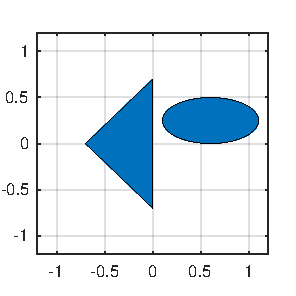
\includegraphics[width=5cm]{figures/rectangle}
\end{minipage}%
\begin{minipage}{0.33\textwidth}
  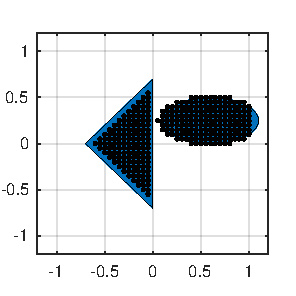
\includegraphics[width=5cm]{figures/rectangle2}
\end{minipage}%
\begin{minipage}{0.33\textwidth}
  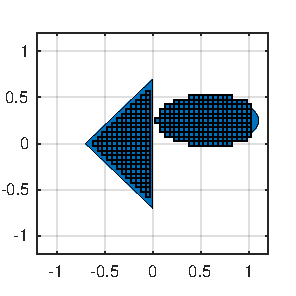
\includegraphics[width=5cm]{figures/rectangle3}
\end{minipage}
\caption{A triangle and an ellipse (displayed on the left) represented with
  {{\tt\small SymbolicSet.hh}} and plotted in MATLAB. In the middle, the grid points are shown,
while on the right the cells associated with the grid points are plotted.}\label{f:symbolicset}
\end{figure}
We use the following code to instantiate an object of {\tt SymbolicSet.hh},
where we use $\segcc{a,b}=\intcc{-1,1}\times\intcc{-1,1}$ and $\eta=(0.05,0.05)$
to define the domain and grid parameter
\begin{lstlisting}[basicstyle=\footnotesize\ttfamily]
#include <array>
#include <iostream>
#include "cuddObj.hh"
#include "SymbolicSet.hh"
int main() {
  Cudd mgr;                                   /* bdd manager to organize the variables */    
  double a[2]={-1,-1};                        /* lower bounds of the hyper rectangle */
  double b[2]={ 1, 1};                        /* upper bounds of the hyper rectangle */
  double eta[2]={0.05,0.05};                  /* grid node distance diameter */
  scots::SymbolicSet sset(mgr,2,a,b,eta);     /* instantiate a SymbolicSet */
\end{lstlisting}
then we use 
\begin{lstlisting}[basicstyle=\footnotesize\ttfamily]
	/* add inner approximation of polytope */
  double H[3*2]={1,0,-1,1,-1,-1};
  double h[3]={0,0.7,0.7};
  sset.addPolytope(3,H,h, scots::INNER);
	/* add outer approximation of ellipse */
  double L[2*2]={2,0 0,4};
  double y[2]={0.6,0.25};
  sset.addEllipsoid(L,y, scots::OUTER);
  sset.writeToFile("symset.bdd");
}
\end{lstlisting}
to add an inner approximation of $P$ and outer approximation of $E$ to the set
{\tt \small sset}. The grid points that are added to the {\tt \small sset} are
illustrated in Fig.~\ref{f:symbolicset}. With the last line, we write the {\tt
\small BDD} representing the grid points in {\tt\small sset} to the file
{\tt\small symset.bdd}. We use the MATLAB interface to visualize the grid points
in MATLAB by 
\begin{lstlisting}[basicstyle=\footnotesize\ttfamily]
>> set=SymbolicSet('symset.bdd');
>> x=set.points;
>> plot(x(:,1),x(:,2),'.')
\end{lstlisting}
In \Cpp, the {\tt\small SymbolicSet} stored in {\tt\small symset.bdd} can simply be read by providing the filename in the constructore. For example, 
\begin{lstlisting}[basicstyle=\footnotesize\ttfamily]
  scots::SymbolicSet newset("symset.bdd");
\end{lstlisting}
reads the {\tt\small SymbolicSet} from file and
instantiates the object {\tt\small newset} with the data stored in {\tt\small
symset.bdd}.


Additionally, we can use the method {\tt\small SymbolicSet::addByFunction} as
illustrated by the listing shown in Fig.~\ref{f:addbyfunction} to add grid
points to a {\tt\small SymbolicSet}. The right
side (of Fig.~\ref{f:addbyfunction}) shows the grid points that are added to
{\tt\small sset}.
\begin{figure}[h]
\begin{minipage}{0.6\textwidth}
\begin{lstlisting}[basicstyle=\footnotesize\ttfamily]
  /* remove all points from the grid */
  sset.clear();
  /* define a function */
  auto f=[](double* x)->bool {
    return (x[0]*x[1]>=0.1);
  };
  /* points with f(x)=1 are added to sset */
  sset.addByFunction(f);          
\end{lstlisting}
\end{minipage}%
\begin{minipage}{0.4\textwidth}
  \centering
  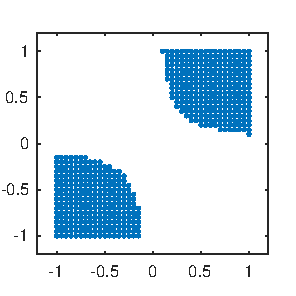
\includegraphics[width=5cm]{figures/rectangle4}
\end{minipage}
\caption{Example usage of {\tt\small
SymbolicSet::addByFunction}.}\label{f:addbyfunction}
\end{figure}

Internally, the grid information is stored in terms of the first grid point and the number
of grid points in each dimension
\begin{lstlisting}[basicstyle=\footnotesize\ttfamily]
double* SymbolicSet::firstGridPoints_
size_t* SymbolicSet::nofGridPoints_
\end{lstlisting}
This information can be access by the method {\tt\small printInfo()}. In the
previous example, the line 
\begin{lstlisting}[basicstyle=\footnotesize\ttfamily]
  sset.printInfo();
\end{lstlisting}
added at the end produces
\begin{lstlisting}[basicstyle=\footnotesize\ttfamily]
First grid point: -1 -1 
Grid node distance (eta)in each dimension: 0.05 0.05 
Number of grid points in each dimension: 41 41 
Number of grid points: 1681
Number of elements in the symbolic set: 570
\end{lstlisting}
The set $S$ (of grid points defined by an instance of {\tt\small SymbolicSet})
is encoded by an instance of a {\tt\small BDD}, which
(in the {\tt CUDD} library) is a \Cpp class that allows one to create, store and manipulate a
function that maps a number of binary variables to $\B:=\{0,1\}$, i.e., 
\begin{IEEEeqnarray*}{c}
  f:\B^m\to \B.
\end{IEEEeqnarray*}
Each grid point $x\in D$ is defined in terms of binary variables $d\in\B^m$ created with
the {\tt CUDD} library.
%In {\tt SCOTS} an element of $d\in\B^m$ evaluates to one, i.e., $f(d)=1$ if and
%only if the grid point $x$ represented by $d$ is an element of the set $S$ represented by {\tt\small SymbolicSet}
By using the {\tt CUDD} library, each {\tt \small BDD} variable obtains
a unique {\tt \small id}. The {\tt\small id}'s of the {\tt\small BDD} variables
that are used in an instance of a {\tt \small SymbolicSet} can by listed by 
\begin{lstlisting}[basicstyle=\footnotesize\ttfamily]
  SymbolicSet::printInfo().
\end{lstlisting}
For example, if we use 
\begin{lstlisting}[basicstyle=\footnotesize\ttfamily]
  sset.printInfo(1);
\end{lstlisting}
at the end of the code in Fig.~\ref{f:addbyfunction}, we obtain 
\begin{lstlisting}[basicstyle=\footnotesize\ttfamily]
Number of binary variables: 12
Bdd variable indices (=IDs) in dim 1: 0 1 2 3 4 5 
Bdd variable indices (=IDs) in dim 2: 6 7 8 9 10 11 
\end{lstlisting}
which tells us the number $(m=12)$  and {\tt id}'s of the {\tt \small BDD} variables 
that are used to encode the grid. 

Each element in $d\in\B^m$ represents a grid
point $\eta\Z^n$. Let us $m_i\in \Z_{>0}$ to denote the number of {\tt\small
BDD} variables that are used to encode the grid points $\intcc{a_i,b_i}\cap \eta_i\Z$ in dimension
$i\in\intcc{1;n}$. Consider the function $\mathtt{id}_i:\N\to \N$ that maps an
index (of the {\tt\small BDD} variable) to the {\tt\small BDD} variable
{\tt\small id}.
Then each component $x_i\in \intcc{a_i,b_i}\cap \eta_i\Z$ of a grid point
associated with an element $d\in\B^m$ is given by
\begin{IEEEeqnarray}{c}\label{e:mapping}
  x_i=p_i+\sum_{j=0}^{m_i-1} d_{\mathtt{id}_i(j)}2^{j}\eta_j=:g_i(d)
\end{IEEEeqnarray}
where $p_i:=\min(\intcc{a_i,b_i}\cap \eta_i\Z)$ is the first grid point for the
component $i\in \intcc{1;n}$.

Consider the example listed in Fig.~\ref{f:addbyfunction}.
Let us use $F:\B^{12}\to \B$ to refer to the
binary function represented by {\tt\small sset.symbolicSet\_}, i.e., the
{\tt \small BDD} instance that encodes $S$, then, in view of the  code in Fig.~\ref{f:addbyfunction}, we have 
\begin{IEEEeqnarray*}{c}
  F(d)=1 \iff g_1(d)\cdot g_2(d)\ge 0.1
\end{IEEEeqnarray*}
where $g_1$ and $g_2$ are defined according to~\eqref{e:mapping}. Note that for
this example $m_1=m_2=6$ and the function $\mathtt{id}_2$ results in
$\mathtt{id}_2(0)=6,\ldots, \mathtt{id}_2(5)=11$.

The individual binary variables $d\in \B^m$ used to represent the set of grid
points in $D$ can be
listed by 
\begin{lstlisting}[basicstyle=\footnotesize\ttfamily]
  sset.printInfo(2);
\end{lstlisting}
For the example in Fig.~\ref{f:addbyfunction}, part of the output is given by 
\begin{lstlisting}[basicstyle=\footnotesize\ttfamily]
000000-000-0  1
000000-00100  1
000000-01-00  1
000000-1--00  1
000001000001  1
000001000101  1
000001000110  1
...
\end{lstlisting}
The symbol {\tt\small-} represent ``don't cares'', which means for example
in the second line that {\tt\small 000000000100} and  {\tt\small 000000100100}
evaluate to $1$. For the last line, we verify
\begin{IEEEeqnarray*}{c}
 g_1(000001000110)\cdot g_2(000001000110)=0.6\cdot 0.2\ge 0.1
\end{IEEEeqnarray*}
The grid point associated with a particular element $d\in\B^m$ is obtained by
the method 
\begin{lstlisting}[basicstyle=\footnotesize\ttfamily]
  SymbolicSet::mintermToElement()
\end{lstlisting}
Here {\tt\small minterm} refers to an integer array of size $m$ and {\tt\small
element} refers to a double array of size $n$. For example, the code 
\begin{lstlisting}[basicstyle=\footnotesize\ttfamily]
  int minterm[12] = {0,0,0,0,0,1,0,0,0,1,1,0};
  double x[2];
  sset.mintermToElement(minterm,x);
  std::cout << x[0] << " " << x[1] << std::endl;
\end{lstlisting}
gives 
\begin{lstlisting}[basicstyle=\footnotesize\ttfamily]
0.6 0.2
\end{lstlisting}
%\begin{lstlisting}[basicstyle=\scriptsize\ttfamily]
%  //double H[sDIM]={-1, -1};//, 1, 1, -1, 1, -1, -1};
%  double H[4*sDIM]={-1, 1, 1, -1, 1, 1,-1, -1};
%  /* add outer approximation of P={ x | H x<= h } form state space */
%  double h[4] = {0.7,0.7,0.7,0.7};
%
%  /* in order to obtain all the necessary information */
%  rec.addPolytope(4,H,h, scots::INNER);
%  
%  rec.writeToFile("rectangle.bdd");
%
%  return 1;
%
%typedef std::array<double,3> state_t; /* state type */
%
%double lb[3]={0,0,-M_PI-0.4}; /* lower bounds */
%double ub[3]={10,10,M_PI+0.4}; /* upper bounds */
%double eta[3]={.2,.2,.2}; /* grid parameter */
%scots::SymbolicSet ss(mgr,3,lb,ub,eta); /* the uniform grid */                           
%ss.addGridPoints(); /* fill the SymbolicSet */ 
%\end{lstlisting}



\subsection{Symbolic Model}
\label{ss:symbolicmodelhh}
The classes {\tt\small SymbolicModel} and {\tt\small SymbolicModelGrowthBound}
implemented in the files {\tt\small ./bdd/SymbolicModel.hh}, respectively,
{\tt\small ./bdd/SymbolicModelGrowthBound.hh} are used to compute 
the transition function $F_2:\bar X_2\times U_2\rightrightarrows \bar X_2$, of
the symbolic model $S_2=(X_2,U_2,F_2)$, see Sec.~\ref{ss:symbolicmodel}.
The transition function can also be considered as relation
$F_2\subseteq \bar X_2\times U_2\times \bar X_2$.
The {\tt\small SymbolicModel} is the base class of {\tt\small
SymbolicModelGrowthBound}, which contains the information about the {\tt\small
SymbolicSet}  representing
\begin{IEEEeqnarray*}{c}
\bar X_2\times U_2\times \bar X_2.
\end{IEEEeqnarray*}
Suppose that the instances {\tt\small ss} and {\tt\small is} of {\tt\small
SymbolicSet} encode the sets $\bar X_2$ and $U_2$, whose domain and grid
parameter are given by
\begin{IEEEeqnarray}{c't'c}\label{e:domaintransitionrelation}
  \segcc{a,b}\subseteq \R^n, \eta\in \R_{>0}^n & respectively & \segcc{c,d}\subseteq \R^m, \mu\in \R_{>0}^m.
\end{IEEEeqnarray}
In order to instantiate an object of {\tt\small SymbolicModel} (or {\tt\small
SymbolicModelGrowthBound}), we first create a copy of {\tt\small ss} to
represent the post $\bar X_2$  with new
{\tt\small BDD} variable {\tt\small id}s by 
\begin{lstlisting}[basicstyle=\footnotesize\ttfamily]
  scots::SymbolicSet sspost(ss,1);
\end{lstlisting}
In this way, the post states in $\bar X_2$ have their own abstract domain.
Afterwards we can instantiate a {\tt\small SymbolicModel} by
\begin{lstlisting}[basicstyle=\footnotesize\ttfamily]
  scots::SymbolicModel abs(ss,is,sspost);
\end{lstlisting}
The {\tt BDD} which represents $F_2\subseteq \bar X_2\times \bar U_2\times \bar
X_2$ is stored in
\begin{lstlisting}[basicstyle=\footnotesize\ttfamily]
  scots::SymbolicModel::transitionRelation_
\end{lstlisting}
and can be accessed via a {\tt\small SymbolicSet} by
\begin{lstlisting}[basicstyle=\footnotesize\ttfamily]
  scots::SymbolicSet tr=abs.getTransitionRelation();
\end{lstlisting}
The domain and grid parameter of {\tt\small tr} follows
from~\eqref{e:domaintransitionrelation} to
\begin{IEEEeqnarray*}{c'c}
  \segcc{a,b}\times \segcc{c,d}\times \segcc{a,b}\subseteq \R^{n+m+n},&
  (\eta,\mu,\eta)\in \R^{n+m+n}_{>0}.
\end{IEEEeqnarray*}


The algorithm, which is implemented in {\tt\small SymbolicModelGrowthBound} to
compute the  transition function of the symbolic model $S_2$ is
listed in Alg.~\ref{alg:transitionfunction}.
\begin{algorithm}[h]
\caption{Computation of $F_2:\bar X_2\times U_2\rightrightarrows \bar
X_2$}\label{alg:transitionfunction}
\begin{algorithmic}[1]
\Require{$\bar X_2$, $U_2$, $\beta$, $\varphi$, $z$, $r=\eta/2$, $\tau$}
\ForAll{$c+\segcc{-r,r}\in \bar X_2$ and $u\in U_2$}
\State $r':=\beta(r+z,u)$
\label{a:l:rpost}
\State $c':=\varphi(\tau,c,u)$
\label{a:l:cpost}
\State   \begin{IEEEeqnarraybox}{c}
    A:=\{x_2'\in X_2\mid \left( c' + \segcc{-r'-z,r'+z} \right) \cap x'_2\neq\emptyset\}
         \end{IEEEeqnarraybox}
\If{$A\subseteq \bar X_2$}
\State $F_2(x_2,u):=A$
\Else
\State $F_2(x_2,u):=\emptyset$
\EndIf
\EndFor
\end{algorithmic}
\end{algorithm}
The computation is based on a growth bound $\beta$ in line~\ref{a:l:rpost}, and the
trajectory of the nominal system $\varphi$
in line~\ref{a:l:cpost}. The mathematical definitions of $\beta$ and $\varphi$
are given in~\eqref{e:GrowthBoundComputation} and above~\eqref{e:growthbound},
respectively.

The functions $\beta$ and $\varphi$ need to be provided by the user. For both
functions, an initial value problem has to be solved. In general, explicit
solutions to such problems do not exist and we are required to work with
numerical approximations obtained by a numerical ODE
solver. For example, in the DC-DC boost converter example in {\tt\small
./examples/bdd/dcdc2} a fixed step size Runge Kutta scheme of order 4 has been
used. The header of the ODE solver is given by
\begin{lstlisting}[basicstyle=\footnotesize\ttfamily]
/* data types for the ode solver */
typedef std::array<double,2> state_type;
typedef std::array<double,1> input_type;
/* function header of the ode solver */
template<class F>
void ode_solver(F rhs, state_type &x, input_type &u, size_t nint, double h);   
\end{lstlisting}
Using the {\tt \small ode\_solver}, a user can define the functions $\varphi$
and $\beta$ in \Cpp as 
\begin{lstlisting}[basicstyle=\footnotesize\ttfamily]
std::function<void(state_type &x, input_type &u)>.
\end{lstlisting}
For example, in {\tt\small ./examples/bdd/dcdc2} we use
\begin{lstlisting}[basicstyle=\footnotesize\ttfamily]
/* we integrate the dcdc ode by 0.5 sec (the result is stored in x)  */
auto  dcdc_post = [](state_type &x, input_type &u) -> void {
  size_t nint=5; /* number of intermediate step size */
  double h=0.1; /* h* nint = sampling time */
  ode_solver(system_ode,x,u,nint,h);
};
/* computation of the growth bound (the result is stored in r)  */
auto radius_post = [](state_type &r, input_type &u) -> void {
  size_t nint=5; /* number of intermediate step size */
  double h=0.1; /* h* nint = sampling time */
  ode_solver(growth_bound_ode,r,u,nint,h);
};
\end{lstlisting}
to provide $\beta$ and $\varphi$ in  line~\ref{a:l:rpost}, respectively, in
line~\ref{a:l:cpost} in Alg.~\ref{alg:transitionfunction}.  Here {\tt\small
system\_ode} and {\tt\small growth\_bound\_ode} are {\tt\small std::function},
which implement the DC-DC boost converter ODE, respectively the ODE associated
with~\eqref{e:GrowthBoundComputation}, see the file {\tt\small dcdc.cc} in
{\tt\small ./examples/bdd/dcdc2}. 

Alternatively, one can use a different ODE solver, for example implemented in
the {\tt\small odeint} library provided within the {\tt\small BOOST} library. An
example that uses an ODE solver provided by the {\tt\small BOOST} library can
be found in {\tt\small ./examples/bdd/boostsolver}. 

Given the functions $\beta$ and $\varphi$ in line~\ref{a:l:rpost}, respectively, in
line~\ref{a:l:cpost} in Alg.~\ref{alg:transitionfunction}, we are ready to call
the method {\tt\small
SymbolicModelGrowthBound::computeTransitionRelation}. For the DC-DC boost converter
example in {\tt\small ./examples/bdd/boostsolver} we use
\begin{lstlisting}[basicstyle=\footnotesize\ttfamily]
  /* copy X and assign new BDD IDs */                                                                                                                                                                                                                                                                                                                           
  scots::SymbolicSet sspost(ss,1);
  scots::SymbolicModelGrowthBound<state_type,input_type> abs(&ss, &is, &sspost);
  /* compute the transition relation */
  abs.computeTransitionRelation(dcdc_post, radius_post);
  /* get the number of elements in the transition relation */
  std::cout << "Number of elements in the transition relation: " << abs.getSize();
\end{lstlisting}
were we instantiate an object of {\tt\small SymbolicModelGrowthBound} with the
{\tt\small SymbolicSet}s {\tt \small ss}, {\tt\small is} and  {\tt\small sspost}.

We can use the method {\tt\small SymbolicSet::writeToFile} to store the transition relation to a file.
For example, in {\tt\small ./examples/bdd/boostsolver} we access the transition relation as {\tt\small SymbolicSet} and write it the file {\tt\small dcdc\_abs.bdd}.
\begin{lstlisting}[basicstyle=\footnotesize\ttfamily]
scots::SymbolicSet tr=abs.getTransitionRelation();
/* write SymbolicSet to file */
tr.writeToFile("dcdc_abs.bdd");
\end{lstlisting}
Note that {\tt\small dcdc\_abs.bdd} not only contains the information of the
transition relation $F_2$, but it also contains the {\tt\small SymbolicSet}
information on $\bar X_2\times U_2\times \bar X_2$. Hence the complete symbolic model
$S_2=(X_2,U_2,F_2)$ can be restored by  
\begin{lstlisting}[basicstyle=\footnotesize\ttfamily]
int main() {
  /* there is one unique manager to organize the bdd variables */
  Cudd mgr;
  /* read SymbolicSet containing the transition relation from file */
  scots::SymbolicSet trset(mgr,"dcdc_abs.bdd");
  /* the first two dimensions correspond to the state alphabet */
  std::vector<size_t> ssdim={1,2};
  scots::SymbolicSet ss(trset,ssdim);
  /* the third dimensions corresponds to the input alphabet */
  std::vector<size_t> isdim={3};
  scots::SymbolicSet is(trset,isdim);
  /* the last two dimensions corresponds to the state alphabet 
   * (containing the post variables) */
  std::vector<size_t> sspostdim={4,5};
  scots::SymbolicSet sspost(trset,sspostdim);
  /* create SymbolicModel */
  scots::SymbolicModel sys(&ss,&is,&sspost);                                                                                                                                                                                                                                                                                                                               
  sys.setTransitionRelation(trset.getSymbolicSet());
  return 1;
}
\end{lstlisting}
see the file {\tt\small ./bdd/examples/boostsolver/dcdcReadFromFile.cc}.



\newpage

\subsection{Controller Synthesis}
\label{ss:controllersynthesis}
The fixed point computations described in Sec.~\ref{ss:fixedpoint} are
implemented in the class {\tt\small FixedPoint}, whose source code can be found  in {\tt\small
./bdd/FixedPoint.hh}. In particular, we use the methods {\tt\small
FixedPoint::reach} and {\tt\small FixedPoint::safe} to compute the maps given in~\eqref{e:con:reach}
and~\eqref{e:con:inv}, respectively. The method  {\tt\small FixedPoint::pre} is
used to compute the map~\eqref{e:pre}.  


Let us demonstrate the usage of {\tt\small FixedPoint} by the example in
{\tt\small ./examples/hscc16/dcdc}. We are given an invariance problem $(S_2,\Sigma_2)$, i.e., $\Sigma_2$ is an invariance specification
associated with $I_2,Z_2$ for some $I_2\subseteq \bar X_2$ and $Z_2\subseteq
\bar X_2\times U_2$. In this example, we use the
{\tt\small SymbolicSet} object {\tt\small ss} to describe $\bar X_2$. Since $Z_2$ is independent of $U_2$ it is sufficient to
make a copy of {\tt\small ss} to describe $Z_2$ as {\tt\small
SymbolicSet}.
We use the code
\begin{lstlisting}[basicstyle=\footnotesize\ttfamily]
	double H[4*2]={-1, 0, 1, 0, 0,-1, 0, 1};
  double h[4] = {-1.15,1.55,-5.45, 5.85};                                                                                                                                                                                                                                                                                                                                  
  /* make a copy of ss */
  scots::SymbolicSet z2(ss);
  z2.addPolytope(4,H,h, scots::INNER);
\end{lstlisting}
to create $Z_2$ and add an inner approximation of the
rectangle illustrated by the red line on the left part of Fig.~\ref{f:dcdcsyn}.
The blue rectangles depict the cells $c+\intcc{-\eta/2,\eta/2}$ in $Z_2$. 
\begin{figure}[h]
\centering
\begin{minipage}{0.45\textwidth}
  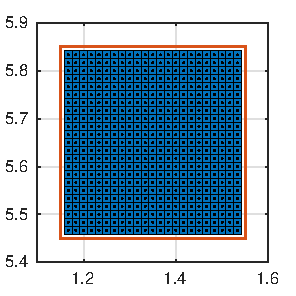
\includegraphics[width=5cm]{figures/dcdcap}
\end{minipage}%
\begin{minipage}{0.45\textwidth}
  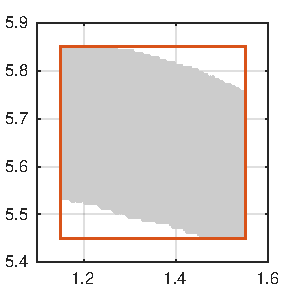
\includegraphics[width=5cm]{figures/dcdcdom}
\end{minipage}
\caption{Left: The set $Z_2$ and its {\tt\small SymbolicSet} representation
  plotted in MATLAB with $\eta=(1/60,1/60)$. Right: The gray shaded region illustrates the domain of the
controller for $\eta=(1/200,1/200)$.}\label{f:dcdcsyn}
\end{figure}

We instantiate an object of {\tt\small FixedPoint} with the symbolic model $S_2$
given by a {\tt\small SymbolicModel} object {\tt\small abstraction}
\begin{lstlisting}[basicstyle=\footnotesize\ttfamily]
  scots::FixedPoint fp(&abstraction);
\end{lstlisting}
The fixed point algorithms in {\tt\small FixedPoint} directly operate on the
{\tt\small BDD} representing the {\tt\small SymbolicSet}. Hence, we first
extract the {\tt\small BDD} from {\tt\small z2} and then use the method {\tt\small FixedPoint::safe} to compute the map~\eqref{e:con:inv} by
\begin{lstlisting}[basicstyle=\footnotesize\ttfamily]
  /* the fixed point algorithm operates on the BDD directly */
  BDD Z = safe.getSymbolicSet();
  BDD C = fp.safe(Z);
\end{lstlisting}
In order to store the result and access the controller from within MATLAB, we
interpret the map~\eqref{e:con:inv} as set $H'_c\subseteq \bar X_2\times U_2$
and create a {\tt\small SymbolicSet} object to store the controller to the file {\tt\small dcdc\_controller.bdd}
\begin{lstlisting}[basicstyle=\footnotesize\ttfamily]
	scots::SymbolicSet controller(ss,is);                                                                                                                                                                                                                                                                                                                                    
  controller.setSymbolicSet(C);
  controller.writeToFile("dcdc_controller.bdd");
\end{lstlisting}
Now the set $H_c'$ can be simply accessed form MATLAB using the MATLAB class {\tt\small SymbolicSet}. For example, with\footnote{Recall that the directory {\tt ./mfiles} needs to be added to the MATLAB path, see Sec.~\ref{s:req}.}
\begin{lstlisting}[basicstyle=\footnotesize\ttfamily]
>> con=SymbolicSet('dcdc_controller.bdd',[1 2]);
>> x=con.points;
>> plot(x(:,1),x(:,2),'.')
\end{lstlisting}
we load the set $H_c'$ as {\tt\small SymbolicSet} form the file {\tt\small
dcdc\_controller.bdd} and plot its domain, see the right part of Fig.~\ref{f:dcdcsyn}. By using the second argument {\tt\small [1 2]} in the
constructor, we only read the points in $H_c'$ projected onto the first two dimensions, see Sec.~\ref{ss:matlab} for more details.

The control inputs defined by the map $H_c'$ can by accessed by 
\begin{lstlisting}[basicstyle=\footnotesize\ttfamily]
>> x=[1.2 5.6];
>> u=con.getInputs(x);
\end{lstlisting}
If the state $x$ is outside the domain of $H_c'$, i.e., $H_c'(x)=\emptyset$ we obtain
\begin{lstlisting}[basicstyle=\footnotesize\ttfamily]
>> con.getInputs(x)  
Error using SymbolicSet/getInputs (line 94)
The state [1.2 5.5] is not in the domain of the controller stored in:dcdc_controller.bdd
\end{lstlisting}

An example which uses {\tt\small FixedPoint:reach} to solve a reachability specification can be found in {\tt\small ./examples/hscc16/vehicle1}.

Note that the method {\tt\small FixedPoint::pre} can be used to compute the
map~\eqref{e:pre}. Hence, it is quite straightforward to implement more complex
fixed point algorithms to compute controllers to enforce more general
specifications. Let us for example consider the \emph{reach-and-stay} specification $\Sigma_2$ associated with $I_2,Z_2$ given by
\begin{IEEEeqnarray*}{c}
\Sigma_2:=\{(u,x)\in (U_2\times X_2)^{\intco{0;\infty}} \mid x(0)\in I_2\implies
\exists_{t\in\intco{0;\infty}}\forall_{t'\in\intco{t;\infty}}: (x(t'),u(t'))\in Z_2\}.
\end{IEEEeqnarray*}
We can solve the control problem $(S_2,\Sigma_2)$ by the nested fixed point algorithm
\begin{IEEEeqnarray*}{c}
	\mu \bar Y.\nu Y. (\pre(Y)\cap Z_2) \cup \pre(\bar Y)
\end{IEEEeqnarray*}
from which we derive a controller as follows. Let $Y_\infty:=\mu \bar Y.\nu Y.
(\pre(Y)\cap Z_2) \cup \pre(\bar Y)$ and consider the sets
\begin{IEEEeqnarray*}{rCl}
  Y_0&:=&\nu Y. (\pre(Y)\cap Y_\infty)\\
  Y_{i+1}&:=&\nu Y. (\pre(Y)\cap Y_\infty)\cup \pre(Y_i)
\end{IEEEeqnarray*}
then a controller $C$, which solves the control problem $(S_2,\Sigma_2)$ is
given by
\begin{IEEEeqnarray*}{rCl}
H_c(q,x_2)&=&
\begin{cases}
H'_c(x_2)\times \{x_2\} & \text{if } x_2\in Y_\infty\\
U_2\times\{x_2\} & \text{otherwise}
\end{cases}\\
F_c(q,x_2)&=&
\begin{cases}
\{q\} & \text{if } x_2\in Y_\infty\\
\emptyset &  \text{otherwise}
\end{cases}
\end{IEEEeqnarray*}
where the map $H_c'$ is given by 
\begin{IEEEeqnarray*}{rCl}
  H'_c(x_2)=\big\{u\in U \mid F_2(x_2,u)\neq \emptyset \land \big((x_2,u)\in Y_0
  \vee  F_2(x_2,u)\subseteq \pi_{X_2}(Y_{j(x_2)-1)})\big)\big\}.
\end{IEEEeqnarray*}
We implemented the fixed point computation in {\tt\small
./examples/bdd/dcdc2} by using {\tt\small FixedPoint::pre} according to the code
\begin{lstlisting}[basicstyle=\footnotesize\ttfamily]
  /* outer fp variables*/
  BDD X=mgr.bddOne();
  BDD XX=mgr.bddZero();
  /* inner fp variables */
  BDD Y=mgr.bddZero();
  BDD YY=mgr.bddOne();
  /* the controller */
  BDD C=mgr.bddZero();
  /* helper BDD */
  BDD U=is.getCube();
  /* outer iteration */
  for(size_t i=1; XX != X; i++) {
    X=XX;
    BDD preX=fp.pre(X);
    /* inner iteration */
    YY = mgr.bddOne();
    for(size_t j=1; YY != Y; j++) {
      Y=YY;                                                                                                                                                                                                                                                                                                                                                                
      YY= ( fp.pre(Y) & T ) | preX;
    }
    XX=YY;
    /* only add (state/input) pairs whose state is not already in the controller */
    BDD N = XX & (!(C.ExistAbstract(U)));
    C=C | N;
  }
\end{lstlisting}
the controller is stored in the {\tt\small BDD C}. We use the method {\tt\small SymbolicSet::writeToFile} to save the result to the file {\tt\small dcdc\_controller.bdd} by
\begin{lstlisting}[basicstyle=\footnotesize\ttfamily]
  scots::SymbolicSet controller(ss,is);
  controller.setSymbolicSet(C);
  controller.writeToFile("dcdc_controller.bdd");
\end{lstlisting}
A closed loop trajectory of the system is illustrated in
Fig.~\ref{f:reachandstay}. The trajectory is obtained by running the MATLAB file
{\tt\small dcdc.m} in the example directory {\tt\small ./examples/bdd/dcdc2}.
\begin{figure}[h]
	\centering
  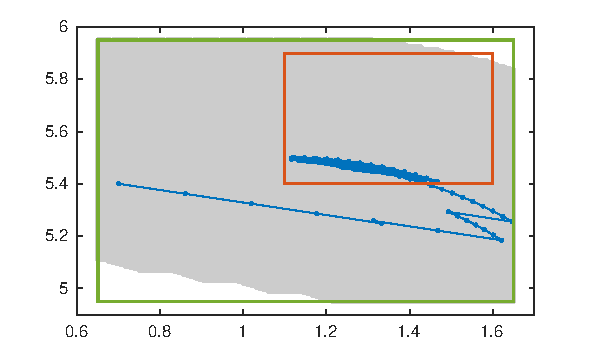
\includegraphics[width=10cm]{figures/dcdcreachandstay}
\caption{Closed loop trajectory of the DC-DC boost converter satisfying
the reach-and-stay specification associated with the red
rectangle.}\label{f:reachandstay}
\end{figure}


\newpage
\subsection{MATLAB Interface}
\label{ss:matlab}
{\tt\small SCOTS} comes with a small {\tt\small mex-file} interface to access {\tt\small
SymbolicSet}s that have been stored using the \Cpp code from MATLAB. The
access of a {\tt\small SymbolicSet} is implemented as a MATLAB
class {\tt\small SymbolicSet} stored in {\tt\small ./mfiles/SymbolicSet.m}.
The MATLAB class provides an interface to the MATLAB commands implemented in the
{\tt\small mex-file}  {\tt\small ./mfiles/mexfiles/mexSymbolicSet.cc}.  In order
to be able to use the MATLAB class {\tt\small SymbolicSet}, the {\tt\small
mex-file} needs to be compiled and added to the MATLAB path, see Sec.~\ref{s:req}. 

Suppose we stored an instance of a {\tt\small SymbolicSet} with domain
$\segcc{a,b}\subseteq \R^n$, grid $\eta\in\R_{>0}^n$ and grid points
\begin{IEEEeqnarray*}{c}
  S\subseteq  (\segcc{a,b}\cap \eta\Z^n).
\end{IEEEeqnarray*}
The MATLAB interface provides three functionalities: 
\begin{itemize}
\item It allows a user
to access the set $S$. For example, for a set $S$ stored in {\tt\small polytope.bdd} (see below) we can use 
\begin{lstlisting}[basicstyle=\footnotesize\ttfamily]
>> P=SymbolicSet('polytope.bdd');
>> x=P.points;
\end{lstlisting}
to load the grid points in $S$ into the MATLAB workspace.
\item It allows a user
to check if an element $x\in\R^n$ is covered by $S$, i.e., 
\begin{IEEEeqnarray*}{c'c}
	\exists_{c\in S}:& x\in c+\segcc{-\eta/2,\eta/2}
\end{IEEEeqnarray*}
Usage:
\begin{lstlisting}[basicstyle=\footnotesize\ttfamily]
>> P.isElement(x);
\end{lstlisting}
\item For a vector $x\in \R^{n_1}$ with
$n_1,n_2\in\intco{1;n}$ and $n_1+n_2=n$, it implements the function 
\begin{IEEEeqnarray}{c}\label{e:setValuedMap}
  S(x)=\{ y\in\R^{n_2}\mid (\intcc{x}_{\eta},y)\in S\}
\end{IEEEeqnarray}
where the components $\hat x_i$ of  $\hat x:=\intcc{x}_{\eta}$ correspond to the
nearest grid point, computed by
\begin{IEEEeqnarray*}{c}
  \hat x_i:=\mathtt{\small std::round}( x_i/\eta_i ) \eta_i
\end{IEEEeqnarray*}
Usage:
\begin{lstlisting}[basicstyle=\footnotesize\ttfamily]
>> P.setValuedMap(x);
\end{lstlisting}
\end{itemize}


Let us consider for example the polytope given by the convex hull $P:=\co(V)$ with
\begin{IEEEeqnarray*}{c}
  V=\left(
      \begin{IEEEeqnarraybox*}[][c]{,r/r/r,}
				0 & -1&  0\\
				 1&  1&   1\\
				-1&  1&   0\\
				 0&  1&  -1 \\
				-1&  0&  -1
      \end{IEEEeqnarraybox*}
\right)
\end{IEEEeqnarray*}
which is illustrated in Fig.~\ref{f:polytope}. We use {\tt\small
SymbolicSet::addPolytope} and {\tt\small SymbolicSet::writeToFile} to compute
an inner approximation of $P$ and to store the result to the file {\tt\small polytope.bdd}.
\begin{figure}[h]
\begin{minipage}{0.68\textwidth}
  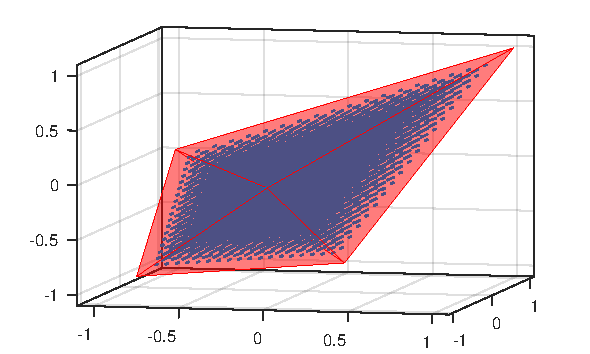
\includegraphics[width=10cm]{figures/polytope}
\end{minipage}%
\begin{minipage}{0.3\textwidth}
  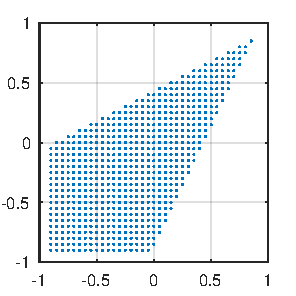
\includegraphics[width=5cm]{figures/polytope1}
\end{minipage}
\caption{}\label{f:polytope}
\end{figure}
Subsequently, we use 
\begin{lstlisting}[basicstyle=\footnotesize\ttfamily]
>> P=SymbolicSet('polytope.bdd');
>> x=P.points;
>> plot3(x(:,1),x(:,2),x(:,3),'.')
\end{lstlisting}
to read and plot the grid points in MATLAB. Optionally, we can provide a list
of indices ${\tt\small idx \subseteq \intcc{1;n}}$, in which case only the grid points projected on the specified indices are loaded. 
For example, with
\begin{lstlisting}[basicstyle=\footnotesize\ttfamily]
>> P=SymbolicSet('polytope.bdd','projection',[1 3]);
>> x=P.points;
>> plot(x(:,1),x(:,2),'.')
\end{lstlisting}
we obtain only a two dimensional vector ${\tt\small x}$ which contains grid points 
\begin{IEEEeqnarray*}{c}
\big\{ (x_1,x_3)\in (\intcc{a_1,b_1}\cap \eta_1\Z)\times (\intcc{a_3,b_3}\cap \eta_3\Z)\mid \exists_{(x_2\in\intcc{a_2,b_2}\cap \eta_2\Z)}: (x_1,x_2,x_3)\in S\big\}.
\end{IEEEeqnarray*}
The outcome of the code listing above is illustrated on the right side of
Fig.~\ref{f:polytope}. This option might be particularly useful, if the set to
be loaded contains a huge amount of grid points. 

The set defined in~\eqref{e:setValuedMap} is implemented in the MATLAB class
method {\tt\small SymbolicSet::setValuedMap}. In the previous
example, we obtain
\begin{lstlisting}[basicstyle=\footnotesize\ttfamily]
>> P.setValuedMap([0.7;.75])     
ans =

    0.7000
    0.6500
\end{lstlisting}
The same functionality is implemented in the method {\tt\small
SymbolicSet::getInputs}. Optionally, a user can provide an index list
${\tt\small idx}\subseteq \intcc{1;n}$. For example, with 
\begin{lstlisting}[basicstyle=\footnotesize\ttfamily]
>> P.setValuedMap([0.7;.75],[3 1]);
\end{lstlisting}
we specify that $0.7$ and $0.75$ correspond to the third, respectively, first coordinate of the $n$-dimensional state space.


%\subsection{Symbolic Set}
%
%\subsection{Symbolic Model}
%
%\subsection{Fixed Point Computations}

\newpage

\part{SPARSE MATRICES BASED IMPLEMENTATION}
~ \\
%\section{To be continued...}
\begin{comment}  
%%%%%%%%%%%%%%%%%%%%%%%%%%%%%%%%%%%%%%%%%%%
 this section currently is not required 
%%%%%%%%%%%%%%%%%%%%%%%%%%%%%%%%%%%%%%%%%%%

\section{Back ground}
~ \\
Sparse Matrix is the Matrix in that most of its elements are zero. See Fig.  ~\ref{f:sparse matrix} as an example of a sparse matrix.
Its structure gives the advantage of using special algorithm to store and manipulate them. Unlike normal matrices which should be stored in the format of $n \times m$ ; for sparse matrices other methods e.g. Dictionary of keys (DIK), List of lists (LIL) and etc. could be used and in hence prevent wasting memory and processing time.

\begin{figure}[h]
\centering
	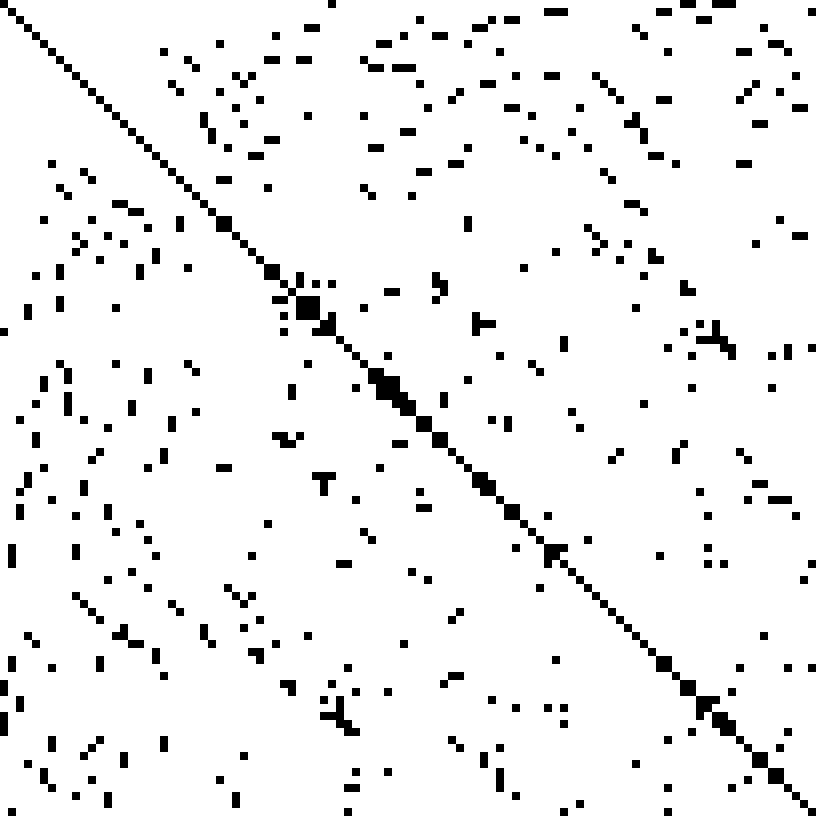
\includegraphics[width=06cm]{figures/Finite_element_sparse_matrix.png}
\caption{A sparse matrix obtained when solving a finite element problem in two dimensions. The non-zero elements are shown in black.}\label{f:sparse matrix}

\end{figure}

 It was initially implemented for 2D matrices but it can be extended to upper dimension too. We will use this matrices for storing the and manipulating of the transition function post or pre elements: 
\begin{IEEEeqnarray*}{c}
F:X \times U\rightrightarrows X
\end{IEEEeqnarray*}

{ \color{red} Also overflow states will be considered as zeros and are not taken into account.}
~ \\ 
\end{comment}
\section{Quickstart}
~ \\
For a quickstart 
\begin{enumerate}
	\item go to one of the examples in
	\begin{lstlisting}[basicstyle=\footnotesize\ttfamily]
	./examples/unicycle      			/* reachability specification */ 
	other examples  						/* will be added */
 
	\end{lstlisting}
	\item read the readme file (if the directory contains one)
	\item edit the {\tt \small Makefile} 
	\begin{enumerate}
		\item adjust the compiler
		\item adjust the directory of the SCOTSROOT 
 \end{enumerate}
	\item compile and run the executable, for example in  {\tt \small ./examples/unicycle} run
\begin{lstlisting}[basicstyle=\small\ttfamily,frame=none]
	$ make
	\end{lstlisting}
	
after  "make"  finished successfully; then run 
	
	\begin{lstlisting}[basicstyle=\small\ttfamily,frame=none]
	$ ./unicycle
\end{lstlisting}

  \item open MATLAB (here we assume that you have already compiled the mex files; in detail you set up the mex compiler in MATLAB as described in Sec.~\ref{s:req}. Also after editing of the make file which is in mfiles folder with concern of MATLAB path you should run this make full too)

    and finally add {\tt \small ./mfiles} to the MATLAB path 
\begin{lstlisting}[basicstyle=\small\ttfamily,frame=none]
  >> addpath(genpath('../../../mfiles')) 
\end{lstlisting}
  \item run the m file, for example in  {\tt \small ./examples/unicycle} run
\begin{lstlisting}[basicstyle=\small\ttfamily,frame=none]
	>> unicycle.m
\end{lstlisting}
\item modify the example to your needs
\end{enumerate}
~ \\
\section{Work Flow Overview- Sparse Matrices}
~ \\
Sparse Matrix is the Matrix in that most of its elements are zero. Its structure gives the advantage of using special algorithm to store and manipulate them. We will use this matrices for storing the and manipulating of the transition function post or pre elements: 
\begin{IEEEeqnarray*}{c}
F:X \times U\rightrightarrows X
\end{IEEEeqnarray*}
Also overflow states will be considered as zeros and are not taken into account.

A short description of the general work flow is given by
\begin{enumerate}
  \item Use the class {\tt\small UniformGrid} to specify 
    \begin{itemize}
      \item the real quantizer symbols $\bar X_2$ 
      \item the input alphabet $U_2$ 
    \end{itemize}
  \item Use the classes {\tt\small AbstractionGB} and {\tt\small TransitionSystem} to compute the transition function $F_2$. You
need to provide 
    \begin{itemize}
      \item the solution of the right-hand-side~\eqref{e:System:c-time} at time $\tau$
      \item and the growth bound~\eqref{e:growthbound} (directly or in terms of $L(u)$
    see~\eqref{e:lipschitz})
    \end{itemize}
  \item Use user defined functions to specify the atomic propositions
    in the specification
  \item Use {\tt \small Game}, and/or {\tt \small ReachabilityGame}, and/or  {\tt \small SafetyGame} to solve the auxiliary control problem $(S_2,\Sigma_2)$ . Other combination of mentioned classes are possible.
  \item Use {\tt\small IO}  to write the result to a file
  \item Optional: Simulate the closed loop in MATLAB by accessing the
    controller saved in the file
\end{enumerate}



% maybe a graph ?

\section{Usage and Implementation Details}


\subsection{Uniform Grid}
\label{ss:Uniform Grid}
~ \\
The source code of the class {\tt\small UniformGrid} is located in {\tt\small ./src/sparse}. For creating, manipulating, and storing of the subsets of grid points this class will be used. It contains a \emph{domain} $\segcc{a,b}\subseteq \R^n$ and a \emph{grid parameter} $\eta\in \R_{>0}^n$. So the domain of the uniform grid is defined by a hyper interval and each grid point $x\in D$ where $D$ :
\begin{IEEEeqnarray*}{c}
  D:=(\intcc{a_1,b_1}\times \cdots\times \intcc{a_n,b_n} )\cap  \eta\Z^n.
\end{IEEEeqnarray*}


is identified with a cell $x+\segcc{-\eta/2,\eta/2}$.
By considering the measurement error bound $z$; the radius of the hyper interval with center of the grid point will be presented as : $ \eta/2 + z$
 
Each grid point is associated with an index. For example by using the domain $\segcc{a,b}\subseteq \R^n$ and grid parameter
    $\eta\in\R^n_{>0}$. For example, to encode a set of grid points in $\intcc{0,2}\times \intcc{0,3} \times \cap  
	(0.5,0.5) \Z^3 $, we can use the following code.
    
    
\begin{lstlisting}[basicstyle=\footnotesize\ttfamily]
#include <array>
#include <iostream>
#include "UniformGrid.hh"
int main() 
{
#define sDIM 2						 /* defining the state space  dimension */
typedef std::array<double,2> state_type; /* defining the state type */


/* construct grid for the state space : */
/* setup the workspace of the synthesis problem and the uniform grid:  */
state_type lb={{0,0}};  	/* lower bounds of the hyper rectangle */ 
state_type ub={{2,3}};    /* upper bounds of the hyper rectangle */
state_type eta={{.5,.5}};   		 /* grid node distance diameter */
scots::UniformGrid<state_type> ss(sDIM,lb,ub,eta);              
return 1;
}
\end{lstlisting}

Figure ~\ref{f:2D-uniformgrid} shows the created grid points which is drawn by help of Matlab interface.

\begin{figure}[h]
\centering
	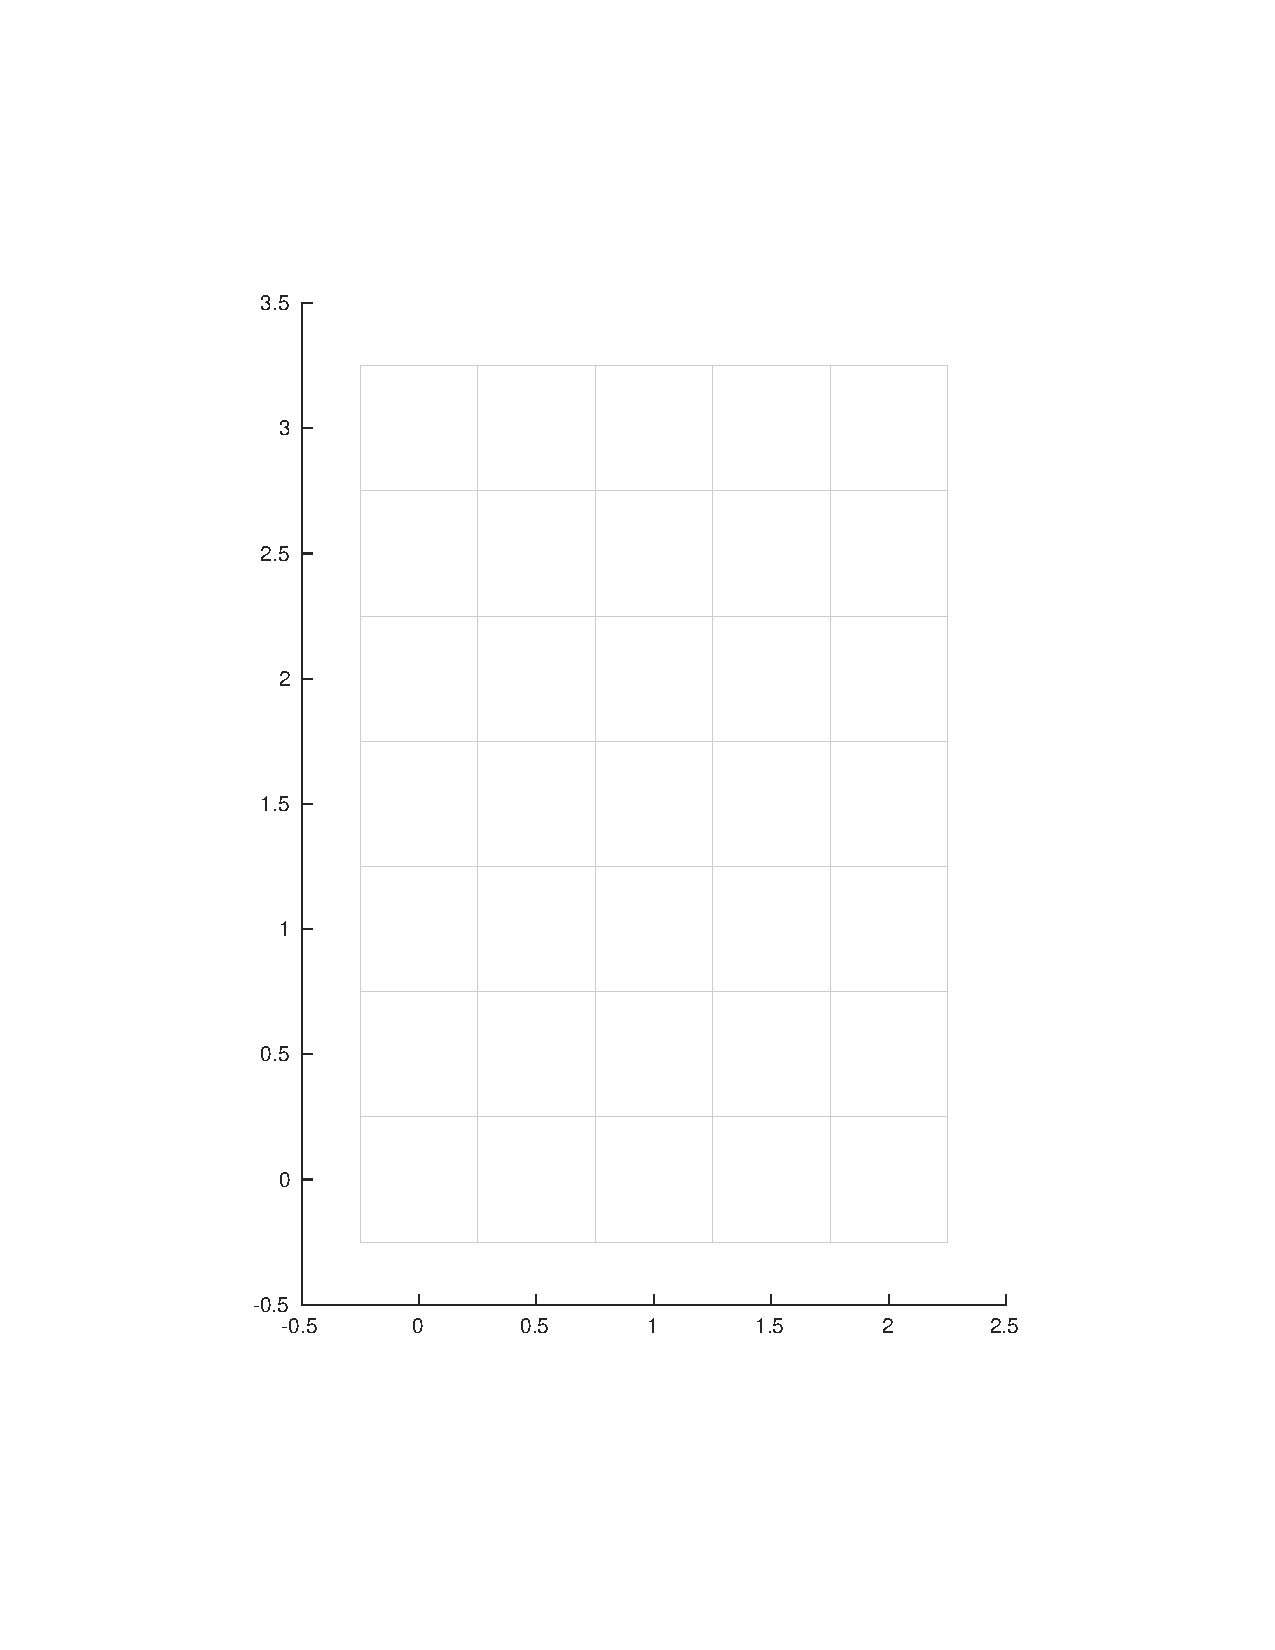
\includegraphics[width=06cm]{figures/manualp1.pdf}
\caption{2D state space example grid point, ilusttrated by help of matlab}\label{f:2D-uniformgrid}

\end{figure}

It is worth to mention that for {\tt\small state\_type} the {\tt\small std::array} has been chosen by user. It is up to user to choose {\tt\small std::array} , {\tt\small std::vector} or other type definition.


Each grid point in SCOTS has an index, Figure  ~\ref{f:index} shows the indexes associated with pre mentioned state space.

\begin{figure}[h]
\centering
	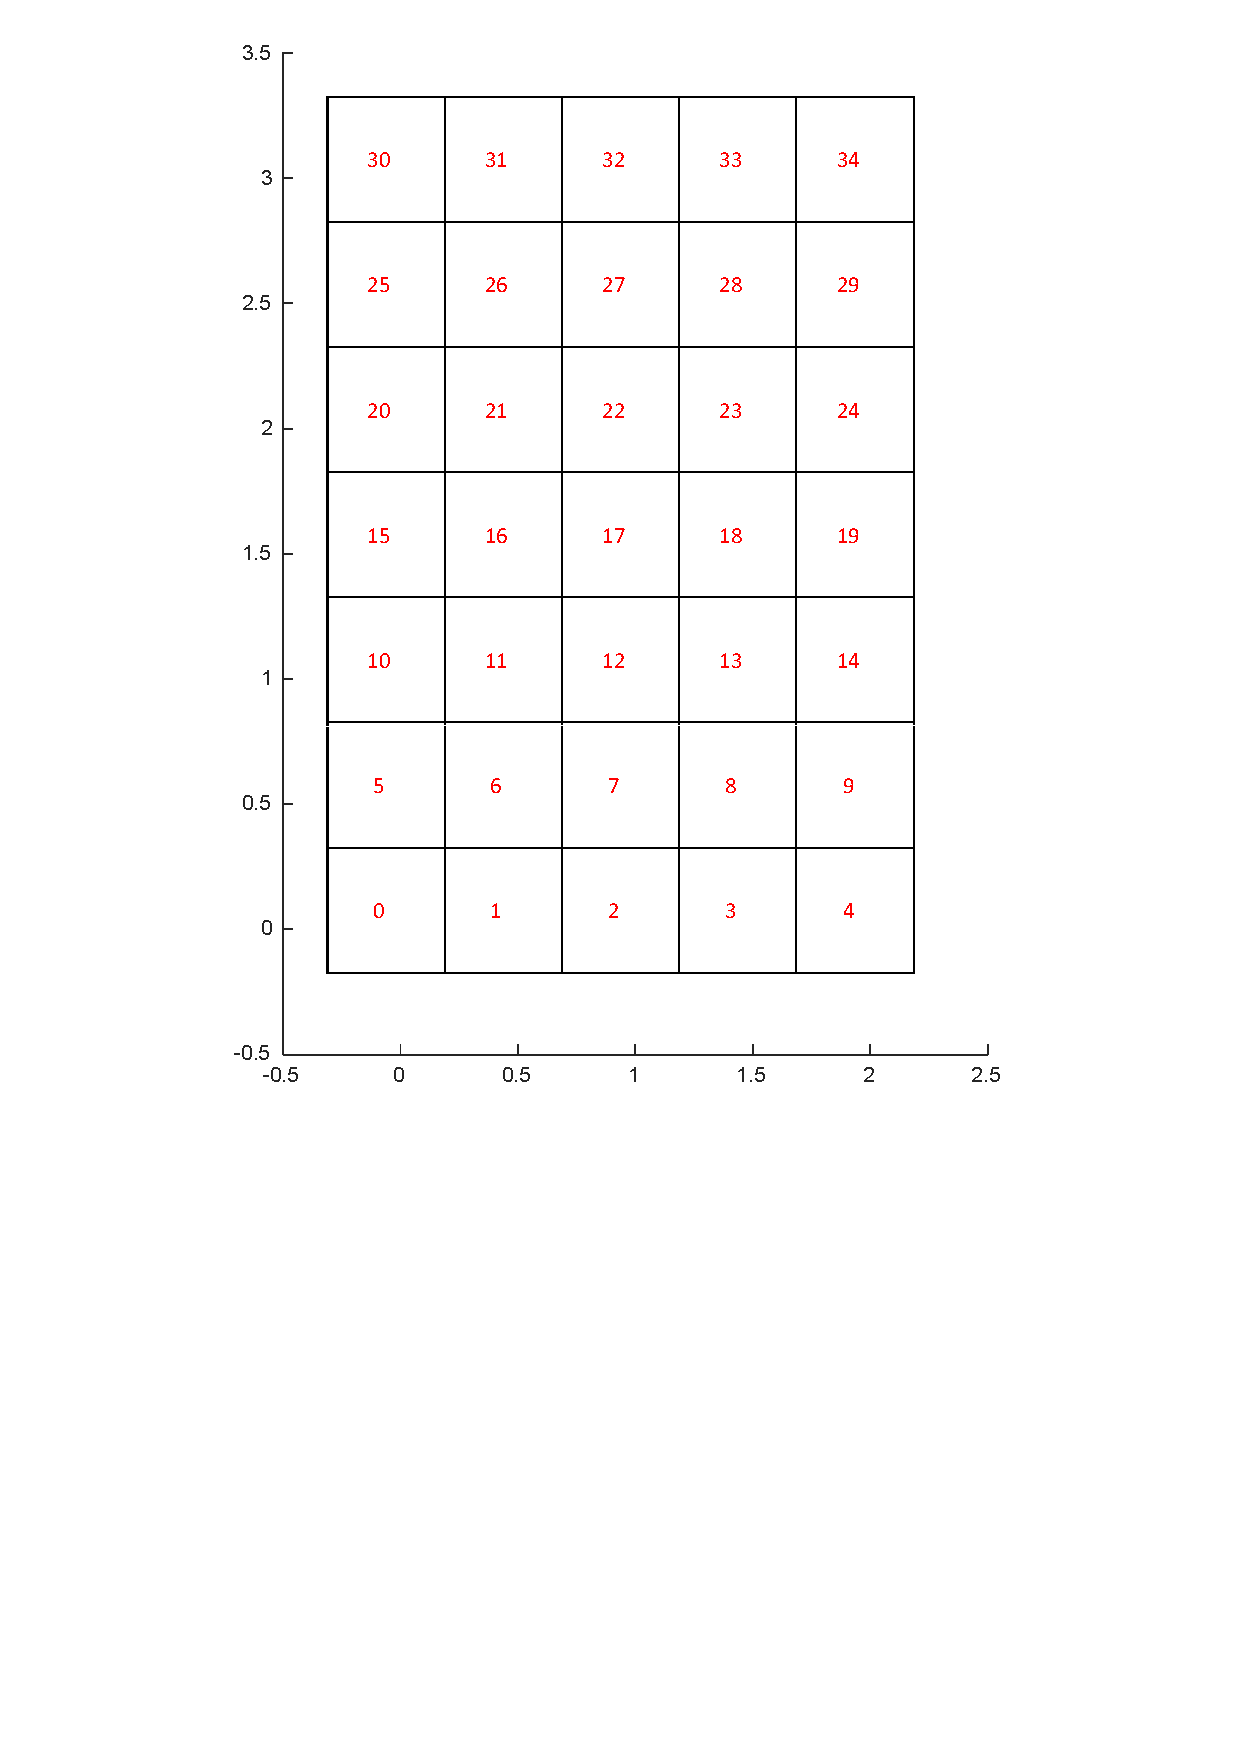
\includegraphics[width=06cm]{figures/manualp2.pdf}
\caption{indexes of 2D state space example grid point}\label{f:index}

\end{figure}

To compute the index {\tt\small idx} associated with a grid point {\tt\small x} we use 
{\tt\small xtoi} and in contrast; to compute the coordinated of the grid point {\tt\small x} associated with the index {\tt\small idx}, {\tt\small itox} will be used. (to memorizing read {\tt\small xtoi} as x to index  and {\tt\small itox}  vice versa).
As an example; assume adding following lines to previous example to gain those data.
\begin{lstlisting}[basicstyle=\footnotesize\ttfamily]
 ss.itox(idx,x);
 ss.xtoi(idx,x);
\end{lstlisting} 
 
 
 
 
 

For more complex example, to encode a set of grid points in $\intcc{0,10}\times \intcc{0,10}\times \intcc{\pi-0.4,\pi+0.4} \cap
    (0.2,0.2,0.1)\Z^3$, we can use the following code. This is an example for creating symbolic input grid points with measurement error $z$.
    
    
\begin{lstlisting}[basicstyle=\footnotesize\ttfamily]
#include <array>
#include <iostream>
#include "UniformGrid.hh"
int main() 
{
#define sDIM 3 						 /* defining the state space  dimension */
typedef std::array<double,3> state_type; /* defining the state type */


/* construct grid for the state space : */
/* setup the workspace of the synthesis problem and the uniform grid:  */
state_type lb={{0,0,-M_PI-0.4}};  	/* lower bounds of the hyper rectangle */ 
state_type ub={{10,10,M_PI+0.4}};    /* upper bounds of the hyper rectangle */
state_type eta={{.2,.2,.1}};   		    /* grid node distance diameter */
state_type z={{.1,.1,0}};   		    /* grid node measurement error bound */
scots::UniformGrid<state_type> ss(sDIM,lb,ub,eta,z);              
return 1;
}
\end{lstlisting}
This is the standard instantiation method to create the symbolic state alphabet $\bar X_2$ with considering $z$. Similar method can be used to create the symbolic input alphabet $U_2$.
\begin{lstlisting}[basicstyle=\footnotesize\ttfamily]
scots::UniformGrid<input_type> is(iDIM,ilb,iub,ieta);
\end{lstlisting}
where this is an example for creating symbolic input grid points without measurement error{\tt\small z}. It is considered that ({\tt\small iDIM,ilb,iub,ieta }) are defined beforehand.



By using the copy constructor, the Uniform Grid variables of original {\tt\small UniformGrid} instance are used for the new one.
\begin{lstlisting}[basicstyle=\footnotesize\ttfamily]
  scots::UniformGrid Nss(ss);  /* Nss and ss have the same abstract domain */
\end{lstlisting}
This option can be used to create atomic propositions to formulate the specification. Also suppose {\tt\small ss} represents $\bar X_2$, then we use the following similar code to create a {\tt\small UniformGrid} to represent a subset of $\bar X_2$
\begin{lstlisting}[basicstyle=\footnotesize\ttfamily]
  scots::UniformGrid subset(ss);   /* subset and ss have the same abstract domain */
\end{lstlisting}


It is possible to create a projection of the grid points in an abstract set onto the specified dimension (so called: [ {\tt\small projectDimension: 1,2,3 ... dim\_ }])
\begin{lstlisting}[basicstyle=\footnotesize\ttfamily]
std::vector<size_t> projectDimension={1,2};
scots::UniformGrid ProjectSet(projectDimension);

\end{lstlisting}

This is beneficial when dimension of the project is more than three and user likes to show specific dimensions on a 2D or 3D diagram.

Similarly, It is possible to create a projection of the grid points in an abstract set which is specified by the argument {\tt\small idxSet} onto the specified dimensions ({\tt\small projectDimension}).

\begin{lstlisting}[basicstyle=\footnotesize\ttfamily]
std::vector<size_t> projectDimension={1,2};
std::vector<size_t> idxSet={1,2,3,5,10,15};
scots::UniformGrid ProjectSet(idxSet, projectDimension);

\end{lstlisting}


Following manipulation are supported in SCOTS.

\begin{lstlisting}[basicstyle=\footnotesize\ttfamily]
UniformGrid::addGridPoints()
/* add all grid points x to the abstract set
 for which the function set(x) == true */
UniformGrid::remGridPoints()	
/* remove all grid points from the abstract set
 for which the function set(x) == true */
UniformGrid::addIndices()
/* add all indices i to the abstract set
 for which the function set(i) == true */
UniformGrid::remIndices() 
/* remove all indices i from the abstract set
for which the function set(i) == true */
UniformGrid::fillAbstractSet() 
/* add all grid points to the abstract set */
UniformGrid::clearAbstractSet() 
/* remove all grid points from the abstract set */
    
\end{lstlisting}

As an example first assume we declared the {\tt\small overflow} grid points before; which this is later used in following code:
\begin{lstlisting}[basicstyle=\footnotesize\ttfamily]
 ss.addGridPoints(overflow);
\end{lstlisting}
then we can add them into the grid points and later consider them as obstacles and write them into a file using {\tt\small IO} see  example unicycle for more detail.

In another example assume after declaration of the {\tt\small Uniformgrid} and all about {\tt\small AbstractSet}, you can use {\tt\small FillAbstractSet} and then write them to the file as problem domain. you will see more about writing to files later.

\begin{lstlisting}[basicstyle=\footnotesize\ttfamily]
 ss.fillAbstractSet();
 scots::IO::writeToFile(&ss,"problemdomain.scs"); 
\end{lstlisting}


Some information related to the Uniform Grid could be accessed by {\tt\small printInfo}. as an example adding 

\begin{lstlisting}[basicstyle=\footnotesize\ttfamily]
ss.printInfo()
\end{lstlisting}
will produce: 
\begin{itemize}
\item Grid node distance $\eta$ in each dimension
\item First grid point
\item Number of grid points in each dimension
\item Number of grid points
\end{itemize}


\subsection{TransitionSystem}
 ~\\
The {\tt\small scots} class {\tt\small TransitionSystem}  is stored in the file  {\tt\small ./src/sparse/TransitionSystem.hh} and contains the transition relation of a transition system. are used to compute 
the transition function $F_2:\bar X_2\times U_2\rightrightarrows \bar X_2$, of
the symbolic model $S_2=(X_2,U_2,F_2)$, see Sec.~\ref{ss:symbolicmodel}.
The transition function can also be considered as relation
$F_2\subseteq \bar X_2\times U_2\times \bar X_2$. ~\cite{RunggerZamani16} The data structure is particularly tailored to be used in the minimal and maximal fixed point computations.
As an example following code will compute the transition System
\begin{lstlisting}[basicstyle=\footnotesize\ttfamily]
scots::TransitionSystem ts;   /* transition system to be computed */
\end{lstlisting}
which is representing
\begin{IEEEeqnarray*}{c}
F_2\subseteq \bar X_2\times U_2\times \bar X_2
\end{IEEEeqnarray*}



\begin{figure} [th]
\centering
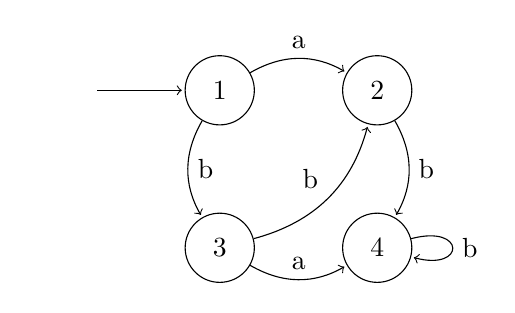
\begin{tikzpicture}[shorten >=1pt,node distance=2cm,on grid,auto] 
  

  \node[state] (1) {1};
  \node[state,draw=none] (d1) [left of=1] {};
  \node[state] (2) [right of=1] {2};
  \node[state] (3) [below of=1] {3};
  \node[state] (4) [below of=2] {4};
 
  \path[->]
    (d1) edge [swap] node[auto] {} (1)
    (1) edge [bend left=30] node {a} (2)
    (2) edge [bend left=30] node {b} (4)
    (3) edge [bend right=30] node  {b} (2)
    (4) edge [loop right] node {b} (4)    
    (1) edge [bend right=30] node {b} (3)
    (3) edge [bend right=30] node {a} (4);
\end{tikzpicture}
\caption{example for transition system}\label{f:4s2i}
\end{figure}

{\color{red} I will explain about the figure example for transition system (figure ~\ref{f:4s2i}) and explain the lists and pre and posts.

.

.
}
Transition system {\tt\small F} regarding the system shown in Figure ~\ref{f:4s2i} will be as 
\begin{IEEEeqnarray*}{c}
F_2\subseteq \bar X_2\times U_2\times \bar X_2 \\
F_2 : {(1,a,2),(a,b,3),(2,b,4),(3,b,2),(3,a,4),(4,b,4)}
\end{IEEEeqnarray*}


............

.....\\
Further calculation will be done with help of {\tt\small AbstractionGB} class where the class {\tt\small Transitionsystem} will be used.
~ \\


\subsection{Abstraction Growth Bound}
~\\
The class {\tt\small AbstractionGB} which is stored in the file 
{\tt\small ./src/sparse/AbstractionGB.hh} is mainly implemented to calculate the Abstraction Growth Bound. This class contains the information of the symbolic model $S_2=(X_2,U_2,F_2)$, means basically 
\begin{itemize}
\item State Space
\item Input Space
\item Transition Function 
\end{itemize}
As first step after computing the Transition System and storing it into {\tt\small ts}, then we can produce abstraction by

\begin{lstlisting}[basicstyle=\footnotesize\ttfamily]
scots::AbstractionGB<state_type,input_type> abs(&ss,&is,&ts);
\end{lstlisting}

{\tt\small ss} and {\tt\small is} has been defined before in subsection ~\ref{ss:Uniform Grid}.
Then we would continue to compute the Transition Relation by using the function {\tt \small computeTransitionRelation} which is implemented as 
\begin{lstlisting}[basicstyle=\footnotesize\ttfamily]
template<class F1, class F2, class F3>
void computeTransitionRelation
	(	F1 &system_post, F2 &radius_post, F3 &overflow, char* cmd="default")

\end{lstlisting}
 as an practical example for unicycle  example; this function will be used in form of: 
 \begin{lstlisting}[basicstyle=\footnotesize\ttfamily]
 abs.computeTransitionRelation(unicycle_post, radius_post,overflow,"preOnly");
 \end{lstlisting}
 
In fact to use the function {\tt\small computeTransitionRelation} you should provide:
\begin{lstlisting}[basicstyle=\footnotesize\ttfamily]
system_post(x,u) 
/* computes the center of the hyper rectangle that containes the attainable set */
radius_post(x,u,z) 
/* computes the radius of the hyper rectangle containing the attainable set */ 
overflow(x,r,z)
/* check if the hyper rectangle with center x, 
and radius r+z intersects with an overflow symbol */
\end{lstlisting}
this could be done with help of ode solver function and providing $\beta$ and $\varphi$ by user. See sections ~\ref{ss:symbolicmodelhh} and ~\ref{ss:GB} for more theoretical detail. {\color{red} here algorithm 1 can be repeated or atleast this part can be explained more}

To get into the detail more; the example of unicycle (available in the path : {\tt\small ./examples/unicycle}) and implementing of ode solver in the scots will be presented in the following:

\begin{lstlisting}[basicstyle=\footnotesize\ttfamily]
/* data types for the state space elements and input space
 * elements used in uniform grid and ode solvers 
 */
typedef std::array<double,3> state_type;
typedef std::array<double,2> input_type;

/* forward declaration of the ode solver */
template<class F>
void ode_solver(F rhs, state_type &x, input_type &u, size_t nint, double h);

/* we integrate the unicycle ode by 0.3 sec (the result is stored in x)  */
auto  unicycle_post = [](state_type &x, input_type &u) -> void {

  /* the ode describing the unicycle */
  auto rhs =[](state_type& xx,  const state_type &x, input_type &u) -> void {
      xx[0] = u[0]*std::cos(x[2]);
      xx[1] = u[0]*std::sin(x[2]);
      xx[2] = u[1];
  };

  size_t nint=5; /* number of intermediate step size */
  double h=0.06; /* h* nint = sampling time */
  ode_solver(rhs,x,u,nint,h);
};

/* computation of the growth bound (the result is stored in r)  */
auto radius_post = [](state_type &r, input_type &u) -> void {
    r[0] = r[0]+r[2]*std::abs(u[0])*0.3;
    r[1] = r[1]+r[2]*std::abs(u[0])*0.3;
};
\end{lstlisting}
as you see in the code 
{\tt\small radius\underline{\hspace{.07in}}post } and {\tt\small unicycle\underline{\hspace{.07in}}post } has been implemented by help of ode solver and previously in section  ~\ref{ss:Uniform Grid} the {\tt\small overflow} has been defined; therefore it is possible now to compute the Abstraction Growth Bound and Transition Relations.
{\color{red} more description is required and should be added}
~ \\
\subsection{Input Output I/O}
~ \\
{\color{red} I will explain following functions and principle of {\tt\small IO} class . or maybe just briefly}
\begin{lstlisting}[basicstyle=\footnotesize\ttfamily]
/* function:  readDimensionFromFile
   * a function to read the dimension of the uniform grid from file */
  /* function:  readMembersFromFile
   * a function to read the uniform grid data from file */
    /* parameters are only read from lines that start with
     * '#key' */
     /* function: writeToFile()
   * ts: TransitionSystem
  /* function: writeToFile()
   * gs: UniformGrid */
    /* function: writeControllerToFile()  (only save the graph)
   * gg: Game
   * filename: name of file */
    /* function: writeControllerToFile()  (save the graph and grid points)
   * ss,is: UniformGrid
   * gg: Game
   * filename: name of file */
     /* function: readFromFile()
   * ts: TransitionSystem
   * filename: name of file */
     /* read the dimension  from file */
    /* read others (controller and ...)  from file */
\end{lstlisting}



\subsection{Other Classes}
~ \\
{\tt\small TicToc} is a class to measure elapsed time based on {\tt\small std::chrono} library. Following code shows an example how to use them.
\begin{lstlisting}[basicstyle=\footnotesize\ttfamily]
TicToc tt;
tt.tic();   /* start */
/* desired process code */
tt.toc();   /* stop */

\end{lstlisting}











{\color{red} It is going on :P }

%\part{THEORETICAL BACKGROUND}
%
%\section{Systems, Composition, Closed Loop}
%
%\section{}


\newpage

\printbibliography

\end{document}
